% % Alice Comments:
% Does the contact force drop once the roughness is implemented?   How are we going to say about the large contact force, for example 5,9 N is a large number for Li4SiO4 pebble? Should I compare Eq. 3.29 with Eq. 3.16? The contact force disappears (or not apparent) in Eq. 3.29? Since there is a quite a significant drop in keff, discussions should be a bit details.  

% DONE Label for Fig. 3-16.  

%  You discuss E after thermal conductance section. What E do you use to get contact force of 5.9 N? 

% DONE I think the arrangement seems good. The title for Chapter 3 may need to change to include fragment study.  Like Construction of a Transient DEM for Solid-Solid Conductance and Packing Alteration Study (or without Construction of)? 

% DONE In Introduction you can then say this forms the basis for further development. Also, you don't use "spend some time" in a scientific paper. 




\chapter{Transient DEM Modeling of Solid-solid Contact Conductance and Packing Changes in Solid Breeder Pebble Beds}\label{ch:modeling-development}


In this chapter thorough descriptions of mechanical and thermal interactions internal to packed beds and their governing equations as implemented with the discrete element method are given. We start with establishing a kinematics framework which simply states that physical granular interactions obey Newton's laws of motion, and the motion of interactions is integrated in time. Contact mechanics models then dictate the normal and tangential forces of interacting grains that feed into the generic kinematic equations; the choice of contact model thus largely dictates the overall behavior of the granular material. Granular heat conductance models are implemented in DEM which, too, is reliant upon the contact force modeling. Application of DEM as a tool for measuring thermomechanical interactions between pebbles for solid breeders is validated \textit{via} numerical experiments to compare effective thermal conductivity with established measurements of effective thermal conductivity of lithium ceramic pebble beds. The contact model we use is based on Hertz's solution for elastic bodies, thus the elastic modulus of the grain is an important property for our models and we experimentally validate the application of Hertz Law; validation is possible with a new phenomenological model for the ceramic pebble elasticities. Lastly a technique for fragmentation modeling and investigate fragments and resettling in numeric ensembles is provided. The DEM model established in this chapter will form the basis for further development of tools for determining temperature distributions in solid breeder pebble beds.

%%%%%%%%%%%%%%%%%%%%%%%%%%%%%%%%%%%%%%%%%%%%%%%%%%%%%%%%%%%%%%%%%%%%%%%%%%%%%%%%%%%%%%%%%%%%%%%%%%%%%%%%%%%%
%%%%%%%%%%%%%%%%%%%%%%%%%%%%%%%%%%%%%%%%%%%%%%%%%%%%%%%%%%%%%%%%%%%%%%%%%%%%%%%%%%%%%%%%%%%%%%%%%%%%%%%%%%%%
%
% new section
%
%%%%%%%%%%%%%%%%%%%%%%%%%%%%%%%%%%%%%%%%%%%%%%%%%%%%%%%%%%%%%%%%%%%%%%%%%%%%%%%%%%%%%%%%%%%%%%%%%%%%%%%%%%%%
%%%%%%%%%%%%%%%%%%%%%%%%%%%%%%%%%%%%%%%%%%%%%%%%%%%%%%%%%%%%%%%%%%%%%%%%%%%%%%%%%%%%%%%%%%%%%%%%%%%%%%%%%%%%
\section{Grain-scale Modeling} \label{sec:modeling-dem}

The observable, macroscopic behavior of particulate, or granular, systems is a complex function of myriad particle interactions. Historically, empirical relationships have been used to describe these systems as if continuous media, \textit{e.g.} the correlations for heat transfer discussed in \Cref{sec:granular-ht-correlations}. But with the advent of the discrete element method by Cundall \& Strack and the acceleration of computing power, it became practical to investigate these granular materials at the particle scale without continuum assumptions \cite{Cundall1979}. With DEM, we track all the particles in the system in a Lagrangian manner. In the ensemble, the kinematics of each particle is tracked and updated based on balances (or imbalances) of forces or energy acting upon the particle. 


%~~~~~~~~~~~~~~~~~~~~~~~~~~~~~~~~~~~~~~~~~~~~~~~~~~~~~~~~~~~~~~~~~~~~~~~~~~~~~~~~~~~~~~~~~~~~~~~~~~~~~~~~~~~
% new subsection
%~~~~~~~~~~~~~~~~~~~~~~~~~~~~~~~~~~~~~~~~~~~~~~~~~~~~~~~~~~~~~~~~~~~~~~~~~~~~~~~~~~~~~~~~~~~~~~~~~~~~~~~~~~~
\subsection{Particle Dynamics}\label{sec:particle-dynamics}

The grains in our system are allowed translational and rotational degrees of freedom. In a packed bed, we can restrict our attention to local forces between particles; neglecting, say, non-contact forces such as, van der Waals, electrostatic, or for the time being any fluid interaction forces. Assuming we know the contact forces acting upon particle $i$, Newton's equations of motion are sufficient to describe the particle kinematics. For translation and rotational degrees of freedom, the equations are:,
\begin{subequations}
\label{eq:newtons-second}
\begin{align}
	m_i  \ddt{\vec{r}_i}   & = m_i\vec{g} + \vec{f}_i \label{eq:newton-translational} \\
	I_i\dt{\vec{\omega}_i} & = \vec{T}_i \label{eq:newton-rotational}
\end{align}
\end{subequations}
where $m_i$ is the particle mass, $\vec{r}_i$ its location in space, $\vec{g}$ is gravity, $I_i$ is the particle's moment of inertia, and $\vec{\omega}_i$ its angular velocity.

The net contact force, $\vec{f}_i$, represents the sum of the normal and tangential forces from the total number of contacts, $Z$, acting on this grain.
\begin{equation}
 	\vec{f}_i = \sum_{j=1}^{Z} \vec{f}_{n,ij} + \vec{f}_{t,ij}
 \end{equation} 
and the net torque, $\vec{T}_i$, is similarly,
\begin{equation}
	\vec{T}_i = -\frac{1}{2}\sum_{j=1}^{Z} \vec{r}_{ij} \times \vec{f}_{t,ij}
\end{equation}

When Cundall \& Strack first proposed the discrete element method, they used a linear spring-dashpot structure which saw normal and tangential forces written as,
\begin{subequations}
\label{eq:dem-forces}
\begin{align}
	\vec{f}_{n,ij} &= k_{n,ij} \delta_{n,ij}\vec{n}_{ij} - \gamma_{n,ij} \vec{u}_{n,ij} 	\label{eq:normal-force} \\
	\vec{f}_{t,ij} &= k_{t,ij} \delta_{t,ij}\vec{t}_{ij} - \gamma_{t,ij} \vec{u}_{t,ij} 	\label{eq:tangential-force}
\end{align}
\end{subequations}
where Cundall \& Strack defined the stiffness coefficients $k$ as constants and local damping coefficients $\gamma$ were proportional to them, $\gamma \propto k$, to allow dissipation of energy and the system to reach an equilibrium. 

Relative normal and tangential velocities, respectively, are decomposed from particle velocities,
\begin{subequations}
\label{eq:dem-velocities}
\begin{align}
	\vec{u}_{n,ij} &= (-(\vec{u}_i-\vec{u}_j)\cdot\vec{n}_{ij})\vec{n}_{ij} \\
	\vec{u}_{t,ij} &= (-(\vec{u}_i-\vec{u}_j)\cdot\vec{t}_{ij})\vec{t}_{ij}
\end{align}
\end{subequations}
with the unit vector $\vec{n}_{ij}$ pointing from particle $j$ to $i$

As in the solution of Hertzian interaction (see \Cref{sec:hertz-theory}), the surfaces of the two particles are allowed to virtually pass through each other (no deformation) resulting in normal and tangential overlaps of,
\begin{subequations}
\label{eq:dem-overlaps}
\begin{align}
	\delta_{n,ij} &= (R_i + R_j) - (\vec{r}_i -\vec{r}_j)\cdot \vec{n}_{ij} \\
	\delta_{t,ij} &= \int_{t_{c,0}}^{t} \vec{u}_{t,ij}\,\mathrm{d}\tau 
\end{align}
\end{subequations}
where the fictive tangential overlap, $\delta_{t,ij}$, is truncated to so the tangential and normal forces obey Coulomb's Law, $\vec{f}_{t,ij} \le \mu_i \vec{f}_{n,ij}$ with $\mu$ as the coefficient of friction of the particle.

Thus the approach of DEM is relatively simple: calculate interaction forces between particles with \Cref{eq:dem-forces} based on the kinematics of velocity and position of interacting particles from \Cref{eq:dem-velocities} and \Cref{eq:dem-overlaps}, respectively, then update the positions based on the forces. As DEM evolved and drew attention of more researchers, more complex formulas governing the spring-dashpot coefficients of \Cref{eq:dem-forces} emerged. But the core approach remained the same and the models all fall into the same family of so-called `soft particle' models of DEM. A well-composed summary of the different DEM force models is given by Zhu\etal.\cite{Zhu2007}

The method used in this work fits into the computational skeleton of Cundall and Strack's method but with non-linear spring-dashpot coefficients defined by simplified Hertz-Mindlin-Deresiewicz model. In this model, the normal-direction stiffness coefficient of \Cref{eq:normal-force} is based on the Hertzian contact law (derived explicitly in \Cref{sec:hertz-theory}). The validity of Hertzian descriptions of normal forces is tested experimentally and reported in \Cref{sec:exp-reduction-factor}.The tangential-direction stiffness coefficient follows from Brilliantov \cite{Brilliantov1996, Zhu2007, Langston1995}. Together, the spring coefficients are,
\begin{subequations}
\begin{align}
	k_{n,ij} &= \frac{4}{3}E_{ij}^*\sqrt{R_{ij}^*\delta_{n,ij}} \\
	k_{t,ij} &= 8 G_{ij}^*\sqrt{R_{ij}^*\delta_{t,ij}}
\end{align}
\end{subequations}
where $E_{ij}^*$ is the pair elastic modulus, $G_{ij}^*$ is the pair bulk modulus, and $R_{ij}^*$ is the relative radius. The terms are defined as,
\begin{subequations}
\begin{align}
	\frac{1}{E^*} &= \frac{1-\nu_1^2}{E_1} + \frac{1-\nu_2^2}{E_2} \\
	\frac{1}{R^*} &= \frac{1}{R_1} + \frac{1}{R_2} \\
	\frac{1}{G^*_{ij}} &= \frac{2(2+\nu_i)}{E_i} + \frac{2(2+\nu_j)}{E_j}
\end{align}
\end{subequations}

Similar to Cundall \& Strack's formulation, damping coefficients, $\gamma$, are included to account for energy dissipated from the collision of two particles \cite{DiRenzo2004, Tsuji1992, Tsuji1993}. Whether the damping coefficient is local or global and the exact form of the coefficient is more important for loosely confined granular systems and dictates the way the system approaches an equilibrium state \cite{Makse2004}. For the case of our tightly packed pebble beds, it suffices to use the efficient form of Refs.\cite{Dippel1996, Makse2004, Brilliantov1996, Zhang2005, Zhu2007},
\begin{subequations}
\begin{align}
	\gamma_n &= \sqrt{5}\beta_\text{diss}\sqrt{m^*k_{n,ij}} \\
	\gamma_t &= \sqrt{\frac{10}{3}}\beta_\text{damp}\sqrt{k_{t,ij} m^*}
\end{align}
\end{subequations}
with $\beta_\text{damp}$ as the damping ratio, and the pair mass, $\frac{1}{m^*} = \frac{1}{m_i} + \frac{1}{m_j}$. For a stable system with $\beta_\text{damp} < 1$, the damping ratio is related to the coefficient of restitution, $e$, as
\begin{equation}
	\beta_\text{diss} = -\frac{\ln{e}}{\sqrt{\ln^2{e}+\pi^2}}
\end{equation}

Systems to be solved by DEM models are therefore well-defined after specifying the few material properties of $E$, $\nu$, $\rho$, and $R_p$ and the interaction properties of $\mu$ and $e$.

Having expressed the contact mechanics of the discrete element method, we now must integrate the kinematic equations of the particles to resolve their evolutions. The most common means of marching in time with DEM is the velocity-Verlet algorithm \cite{Kruggel-Emden2008}. In this algorithm, \Cref{eq:newtons-second} are integrated with half-steps in velocity, full steps in position, and then finally the full step in velocity. In practice, the two half-steps in velocity are often compressed into a single, full step. The computational time integration steps are given in explicit detail in \Cref{sec:dem-stability}. Owing to the explicit nature of the velocity-Verlet algorithm, stability is a constant concern with DEM simulations. Stable, critical time steps and practical means of circumventing unreasonably small time steps are discussed in \Cref{sec:dem-stability}.

A last note. Throughout this work, we required a fully quiesced bed to act as a starting point or demarcate a mechanically steady-state bed. To determine when this occurs, the total kinetic energy of the entire ensemble is monitored and a packed bed is considered to have completely settled once the magnitude of the system's kinetic energy is less than $10^{-8}$. A similar process was independently determined in a similar matter in the work of Ref.~\cite{Silbert2002}. 



%~~~~~~~~~~~~~~~~~~~~~~~~~~~~~~~~~~~~~~~~~~~~~~~~~~~~~~~~~~~~~~~~~~~~~~~~~~~~~~~~~~~~~~~~~~~~~~~~~~~~~~~~~~~
% new subsection
%~~~~~~~~~~~~~~~~~~~~~~~~~~~~~~~~~~~~~~~~~~~~~~~~~~~~~~~~~~~~~~~~~~~~~~~~~~~~~~~~~~~~~~~~~~~~~~~~~~~~~~~~~~~
\subsection{Granular Heat Transfer in DEM}\label{sec:dem-heat-transfer}

In a way analogous to handling particle momentums with Newton's laws of motion, Lagrangian tracking of particle energy is obtained \textit{via} the first law of thermodynamics. Each particle is treated as a single distinct object and thus internal temperature gradients are assumed negligible. The temperature of particle $i$ is governed by
\begin{equation}\label{eq:thermoFirstLaw}
	m_iC_i\dt{T_i} = Q_{s,i} + Q_{i}
\end{equation}
where $m$ and $C$ are the mass and the specific heat of the solid, respectively. Heat generation inside the particle is input with $Q_{s}$ and the total heat transferred to/from particle $i$ \textit{via} conduction to all, $Z$, neighboring particles, is
\begin{equation}
	Q_i = \sum_{j=1}^Z Q_{ij}
\end{equation}

Assuming the particles are spherical, smooth, elastic, in vacuum, and we neglect radiation transfer between them, for two particles at temperatures $T_i$ and $T_j$, we quantify the amount of energy transferred between them with a contact conductance, $H_c$:
\begin{equation}\label{eq:pebble-conduction-heat-transfer}
    Q_{ij} = H_{c}(T_i - T_j)
\end{equation}

Batchelor \& O'Brien\cite{Batchelor1977} developed a formulation of similar form and then made a brilliant observation that ``\textit{when the radius of the circle of contact is so large that the heat flux through the thin annular matrix layer is negligible by comparison with that through the contact circle, the distribution of temperature inside the two particles is approximately the same as that of the velocity potential in irrotational flow of incompressible fluid through a circular hole in a plane wall.}'' With the analogy, they made use of the fluid flow solution to write the total heat flux across the circle of contact as \Cref{eq:pebble-conduction-heat-transfer} with heat conductance 
\begin{equation}\label{eq:batchelor-pebble-conductance}
    H_c = 2k_sa
\end{equation}
where $k_s$ is the conductivity of the contacting solids and $a$ is the radius of contact. Because we have assumed smooth, elastic, spherical solids, with Hertz theory (see \Cref{sec:hertz-theory}), contact radius can be found as a function of contact normal force, $F_n$,
\begin{equation}
    a =  \left(\frac{3}{4}\frac{R^*}{E^*}\right)^{1/3}F_n^{1/3} 
\end{equation}
where, as before, $\frac{1}{E^*} = \frac{1-\nu_1^2}{E_1} + \frac{1-\nu_2^2}{E_2}$ and $\frac{1}{R^*} = \frac{1}{R_1} + \frac{1}{R_2}$. 

In the development of \Cref{eq:batchelor-pebble-conductance}, Batchelor \& O'Brien had assumed the two contacting spheres to be of equal conductivity, $k_s$. Cheng\etal\cite{Cheng19994199} proposed a slightly modified conductance which allows for contacting materials of different thermal conductivity. They give,
\begin{equation}\label{eq:cheng-modification-batchelor}
    H_c = 2k^*a = 2k^* \left(\frac{3}{4}\frac{R^*}{E^*}\right)^{1/3}F_n^{1/3}
\end{equation}
where $\frac{2}{k^*} = \frac{1}{k_i} + \frac{1}{k_j}$. As well as being a more general, flexible formulation, the models analyzed by Cheng\etal\cite{Cheng19994199} are in good agreement with experiments.

The condition for validity of Batchelor \& O'Brien's formulation of \Cref{eq:batchelor-pebble-conductance} is in the limit where $\Psi \rightarrow \infty$, where \cite{Batchelor1977}
\begin{equation}\label{eq:conductance-validity-fluid}
    \Psi = \frac{a}{R^*} \kappa
\end{equation}
The term $\frac{a}{R^*}$, from \Cref{sec:hertz-theory}, is necessarily less than 1 for Hertz theory to be applicable. Thus for fluid in vacuum, the condition is identically satisfied but we must consider inaccuracies if we introduce an interstitial fluid with low conductivity ratios; for lithium ceramics in helium, the ratio is approximately $\kappa \approx 10$.

We step back from contact of a single pair of particles and consider a particle in an ensemble with many contacts. We must again consider the validity of applying \Cref{eq:cheng-modification-batchelor} at each contact. Vargas and McCarthy\cite{Vargas2002a}, propose introducing a conduction Biot number to relate resistance of heat transfer internal to a particle with resistance between particles,
\begin{equation}
    \Bi_c = \frac{H_c}{k^* d_p} = 2\frac{a}{d_p}
\end{equation}

Then if $\Bi_c \ll 1$, the individual energy transferred between each point of contact can be decoupled. The Biot number criteria is already satisfied for Hertz theory to be valid; having assumed that $\frac{a}{d_p} \ll 1$. Therefore the total heat transferred out of a single particle with $Z$ contacts, due to contact conductance, is the summed contribution of individual contacts, 
\begin{equation}
    Q_i = \sum_j^Z Q_{ij}
\end{equation}

For the case when we do \textit{not} have a perfectly smooth elastic sphere, we use the approach of Bahrami\etal, introducing a joint thermal resistance to develop a modified heat conductance term. Bahrami\etal\cite{Bahrami2004} use a joint thermal resistance of the superposition of macroscopic and microscopic influences; the thermal joint resistance is
\begin{equation}
	R_j = R_s + R_L
\end{equation}
where the subscript $L$ refers to macroscopic variables and $s$ refers to microscopic ones. Bahrami\etal~used the constriction formulation of Yovanovich\etal~to express the macroscopic resistance as\cite{Yovanovich1976}
\begin{equation}
	R_L = \frac{(1-a/R^*)^{3/2}}{2k_sa}
\end{equation}
If the contact of the two materials obeys Hertz contact law, then $a/R^* \ll 1$ and the above becomes
\begin{equation}\label{eq:macro-thermal-resistance}
	R_L = \frac{1}{2k_sa}
\end{equation}
which matches the heat conduction form of Batchelor \& O'Brien\cite{Batchelor1977}, \Cref{eq:batchelor-pebble-conductance}.

To determine the thermal resistance of the asperities in contact, Bahrami\etal~used a superposition of many cylindrical constrictions inside of the contact area. The result is given in \cite{Bahrami2004} as
\begin{equation}
	\psi_s^* = \begin{cases}
	\left(\frac{\pi H'R^{*2}}{F} \right)^s 										& F_c = 0\\
	(R^*/a)^2(H'/P_0)^s(1+s\gamma) 										& F \le F_c\\
	(H'/P_{0,c})^s(1+s\gamma_c)+\left[\frac{\pi H'R^{*2}}{(F-F_c)}\right]^s				& F\ge F_c
	\end{cases}
\end{equation}
where $\psi_s^*$ is a non-dimensional form of the surface roughness thermal resistance, defined as $\psi_s^* = 1.25\pi R^{*2}k^*(m/\sigma)\psi_s$, $k^*$ is the harmonic mean of contact grains thermal conductivity, $H'$ is the Vicker's microhardness value, $F$ is the contact force, $P_0$ is the maximum pressure of contact, $s$ is a parameter based on the hardness constants, $\gamma = 1.5(P_0/P_{0,H})(a/a_H)^2-1$, $F_c$ is the critical force where $a = R^*$, $\gamma_c$ is the value of $\gamma$ at the critical force, $m$ is the mean absolute surface slope, and $\sigma$ is the root-mean-square (rms) surface roughness. For Hertzian contact, $\gamma = 0.5$.

Antonetti\etal~ proposed a correlation for mean absolute surface slope related to surface asperities as\cite{Antonetti1984}
\begin{equation}\label{eq:m-of-sigma}
	m = 0.125(\sigma\times10^6)^{0.402}
\end{equation}
where the range of applicability of surface roughness is \SI{0.216E-6}{\meter}$\le \sigma <$ \SI{9.6E-6}{\meter}. Thus the term $\sigma/m = 0.031\sigma^{0.598}$

For Hertzian contacts of the non-conforming ceramic materials, $F \ll F_c$, thus we consider only that case to write
\begin{equation}
	R_s = \frac{(R^*/a)^2(H'/P_0)^s(1+s/2)}{1.25\pi R^{*2}k^*(0.031\sigma^{0.598})}
\end{equation}
or
\begin{equation}\label{eq:thermal-resistance-pressure}
	R_s = \frac{(H'/P_0)^s(1+s/2)}{1.25\pi a^2k^*\left(0.031\sigma^{0.598}\right)}
\end{equation}
For Hertzian contact, the maximum pressure is given by \Cref{eq:hertzian-pressure}. It is
\begin{equation*}
	P_0 = \frac{2E^*\delta_n}{\pi a}
\end{equation*}
Furthermore, as noted by Bahrami\etal, the parameter $s$ is in the range of $0.95\le s\le 0.97$. Therefore it is approximated as $s=0.96$ here. The thermal resistance of \Cref{eq:thermal-resistance-pressure} is rewritten in a simplified form,
% \begin{equation}
% 	R_s = \frac{\pi^{s-1}}{1.25(2^s)}\left(\frac{H'}{E^*}\right)^s\frac{1+s/2}{k^*\delta_n^s}\left(\frac{\sigma}{m}\right)a^{s-2}
% \end{equation}
\begin{equation}\label{eq:micro-thermal-resistance}
	R_s = \left(\frac{H'}{E^*\delta_n}\right)^{0.96}\left(\frac{\sigma}{m}\right)\frac{1}{1.720k^*a^{1.04}}
\end{equation}

The macroscopic and microscopic thermal resistances given in \Cref{eq:macro-thermal-resistance} and \Cref{eq:micro-thermal-resistance}, respectively, are combined to give the total joint thermal resistance of
\begin{equation}
	R_j = \left(\frac{H'}{E^*\delta_n}\right)^{0.96}\frac{0.031\sigma^{0.598}}{1.720k^*a^{1.04}} + \frac{1}{2k^*a}
\end{equation}
and the total thermal conductance between the two grains, $H_j = 1/R_J$, is
\begin{equation}\label{eq:micro-macro-conductance}
	H_j = \left[\left(\frac{H'}{E^*\delta_n}\right)^{0.96}\frac{0.031\sigma^{0.598}}{1.720k^*a^{1.04}} + \frac{1}{2k^*a}\right]^{-1}
\end{equation}

In the limit of zero roughness, the first term inside the bracket tends to 0 and the conductance is simply the Batchelor \& O'Brien form with Hertzian assumptions of perfectly smooth elastic spheres. In our DEM model, we employ a flag to choose between the simple smooth assumption for heat conductance, \Cref{eq:batchelor-pebble-conductance}, or the more advanced conductance equation, \Cref{eq:micro-macro-conductance}, if we have known hardness and roughness properties for ceramics. In practice, the hardness and roughness properties are, as yet, unknown for lithium ceramic materials and most studies in this work are done with smooth sphere approximation.

%In the LIGGGHTS source code file `fix\_heat\_gran\_conduction.cpp', the macroscopic thermal resistance is incorporated into the heat conductance term. To include the microscopic term, we simply need information on the $H'$, $\sigma$, and $m$. All other terms of \Cref{eq:micro-macro-conductance} are available to the code.




\subsubsection{Thermal Expansion}
The stresses which will act upon the solid breeder volume during operation of the fusion reactor arise from the differential rate of thermal expansion from the highly heated ceramic volume and the relatively cool structural container. Moreover, thermal settling motion is observed in pebble beds with cyclic heating \cite{Tanigawa:2010cr, Vargas2007, Chen2009, Divoux2008}. Both of those phenomena originate from effects of thermal expansion of individual grains in the ensemble. Therefore, we introduce a simple thermal expansion method into the DEM structure that updates the diameter of each particle as,
\begin{equation}
	d_{p,i} = d_{p_0,i}\left[1+\beta_i\left(T_i - T_0\right)\right]
\end{equation}
where $\beta_i$ is the thermal expansion coefficient (in units of \SI{1}{\per\kelvin}), $T_i$ is the temperature of the pebble at the current step, and $d_{0,i}$ is the initial diameter of the pebble at temperature $T_0$. The update of pebble diameter based on thermal expansion could be computed at every time step as it is not computationally expensive. Nevertheless, flexibility in the code allows computation at an arbitrary interval of time, typically every $\frac{N}{\Delta t} = \frac{10^4}{10^{-7}}$ in most models of ceramic pebble beds).



%~~~~~~~~~~~~~~~~~~~~~~~~~~~~~~~~~~~~~~~~~~~~~~~~~~~~~~~~~~~~~~~~~~~~~~~~~~~~~~~~~~~~~~~~~~~~~~~~~~~~~~~~~~~
% new subsection
%~~~~~~~~~~~~~~~~~~~~~~~~~~~~~~~~~~~~~~~~~~~~~~~~~~~~~~~~~~~~~~~~~~~~~~~~~~~~~~~~~~~~~~~~~~~~~~~~~~~~~~~~~~~
\subsection{Numerical Implementation of DEM}\label{sec:dem-solver}

The primary computational tool used in this study is LAMMPS (Large-scale Atomic/Molecular Massively Parallel Simulator) \cite{Plimpton1995}, a classical molecular dynamics code. The package of code, maintained by Sandia National Labs (http://lammps.sandia.gov), has many features making it particularly attractive for our use of granular material simulations. LAMMPS is open-source and written in highly-portable C++ allowing customization of any core modeling feature. LAMMPS runs with distributed-memory message-passing parallelism (MPI) and provides simple control (manual or automatic) of the spatial-decomposition of simulation domains for parallelizing. Perhaps most importantly, LAMMPS provides an efficient method for detecting and calculating pair-wise interaction forces; the largest consumer of run-time in the DEM algorithm \cite{Plimpton1995}. We build the LAMMPS core as a library to allow coupling LAMMPS features to other numerical tools. The scripting language of Python (Python 2.7) to write parent routines that pass information between LAMMPS objects while accessing all of Python's numeric and scientific libraries (\textit{e.g.} NumPy and SciPy). 

LAMMPS by default provides a rudimentary method of modeling of granular particles (the term `granular' in LAMMPS vernacular simply differentiates the discrete element of molecules or atoms from larger-scale granular particles of powders or pebbles); LAMMPS has been used for studying granular material since at least 2001 when Silbert\etal~studied granular flow on inclined planes \cite{Silbert2001}. However, the usefulness of LAMMPS for studying granular systems was greatly enhanced by LIGGGHTS (LAMMPS Improved for General Granular and Granular Heat Transfer Simulations), a suite of modules included on top of LAMMPS. LIGGGHTS has many academic and industrial contributors from around the world, with the code maintained as open-source by DCS Computing, GmbH.

Briefly, some notable features that LIGGGHTS brings to the LAMMPS environment include: built-in Hertz/Hooke pair styles with shear history, mesh importing for handling wall geometry, moving meshes, stress analysis of imported meshes, a macroscopic cohesion model, a heat transfer model, and improved dynamic load balancing of particles on processors\cite{Kloss2011,Kloss2012}. Both LIGGGHTS and LAMMPS are distributed under the open-source codes under terms of the Gnu General Public License.\cite{FreeSoftwareFoundationInc.2007} LIGGGHTS is compiled with modified source files of heat transfer to account for the introduction surface roughness given in \Cref{eq:micro-macro-conductance}.




\subsection{Benchmarking Solid-Solid Conductance Models for Pebble Beds}\label{sec:dem-benchmark}
For validation, we will compare numeric calculations of effective thermal conductivity to the few experimental campaigns which measured effective thermal conductivity of packed beds in vacuum. For comparison, in \Cref{fig:keff-pressure}, we saw the effective thermal conductivity of a pebble bed, in near-vacuum conditions, is measured by Enoeda\etal~as approximately $\keff = \SI{0.2}{\watt\per\meter\per\kelvin}$ for \lis at \SI{517}{\celsius}. Aquaro \& Zaccari also measured the effective conductivity in vacuum, over a range of external pressures.\cite{Aquaro2007} Their results are reproduced in \Cref{fig:keff-aquaro}. The effective conductivity of \lit~pebble beds are seen to increase from approximately $\keff = \SI{0.2}{\watt\per\meter\per\kelvin}$ to $\keff = \SI{0.3}{\watt\per\meter\per\kelvin}$ over the range of external pressures, \SI{0}{\mega\pascal} to \SI{7}{\mega\pascal}.
\begin{figure}[ht]
\centering
    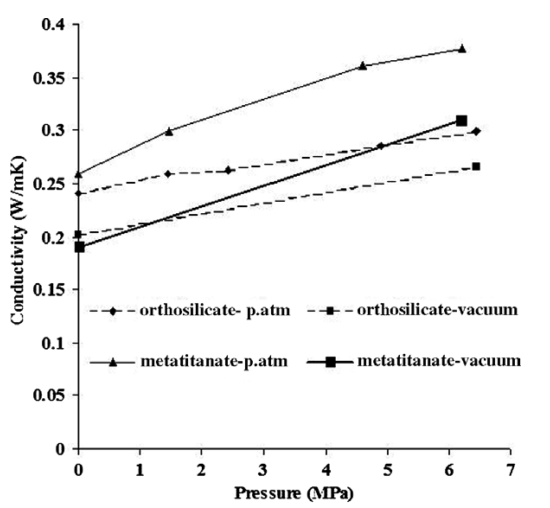
\includegraphics[width=\singleimagewidth]{figures/aquaro.png}
    \caption{Effective conductivity of \lit~and \lis~in air and vacuum environment conditions. Reproduced from Ref \cite{Aquaro2007}.}
    \label{fig:keff-aquaro}
\end{figure}
The solid-solid conductance modeling of DEM can be seen as the vacuum limit when no influence of interstitial purge gas is present; the results of DEM should therefore then be in the range of \SIrange{0.2}{0.3}{\mega\pascal}. 

A recent thermal DEM study has been performed by Gan\etal~which analyzed temperature profiles in pebble bed regions reflecting the European design of helium-cooled pebble bed.\cite{An20072233} In their work, they use the more generic form of heat conductance provided by Batchelor \& O'Brien,\cite{Batchelor1977}
\begin{equation}\label{eq:gan-dem-hc}
H_c = 2\pi\frac{k_s}{\kappa}R^* \mathscr{H}(\kappa,\Psi)
\end{equation}
where $\kappa = k_s/k_g$ as defined above; $\mathscr{H}(\kappa,\Psi)$ is a function of (i) the flux across contact circle, (ii) the difference between the flux across the matrix layer and the total flux between particles in point contact, and (iii) the conductivity ratio $\kappa$. In the limit of $\Psi\rightarrow\infty$ (see \Cref{eq:conductance-validity-fluid}), $\mathscr{H} \rightarrow \frac{\kappa a}{\pi R^*}$ and thus \Cref{eq:batchelor-pebble-conductance} is recovered.

For the case of $\phi = 0.645$, the temperature profile for mono-sized pebbles is reproduced in \Cref{fig:gan-temp-profile-tdem}. 
\begin{figure}[ht]
\centering
    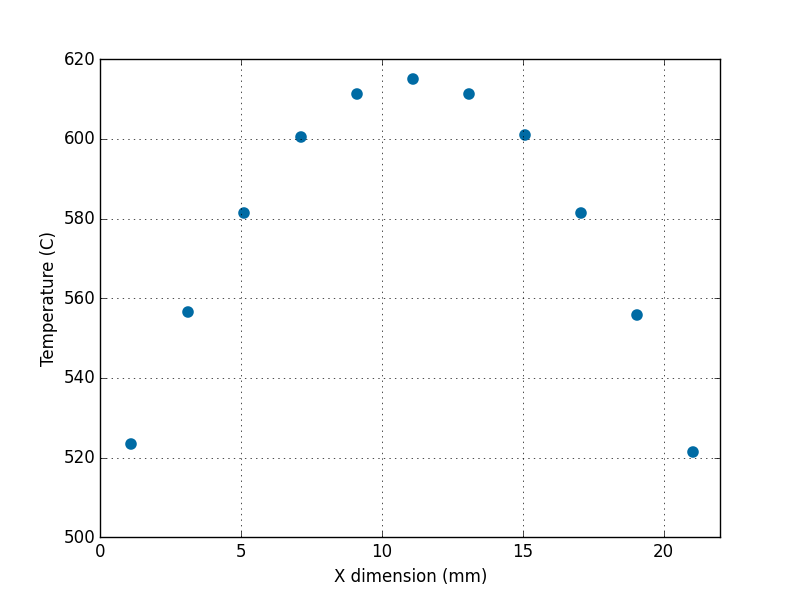
\includegraphics[width=\singleimagewidth]{figures/gan-temp-profile-tdem.png}
    \caption{Temperature profile across a pebble bed from Ref.\cite{An20072233}}
    \label{fig:gan-temp-profile-tdem}
\end{figure}

An effective thermal conductivity can be calculated from the data given by Gan\etal~and using \Cref{eq:keff-formulation}. For the case of $\phi = 0.645$, an effective thermal conductivity is found to be $\keff = \SI{4.37}{\watt\per\meter\per\kelvin}$. In the heat conductance term used by Gan\etal, contribution of helium is accounted for in near-contact regions of pebbles and thus the effective thermal conductivity determined from these beds should be higher than the values of vacuum, yet the value of \SI{4.37}{\watt\per\meter\per\kelvin} is exceedingly high, given the stress state in the pebble bed after heating is calculated as only \SI{5.7}{\mega\pascal}. The effective conductivity was not reported in paper of Gan\etal~and consequently no discussion on why the value is so large is given.

To validate the heat transfer capabilities of our DEM models, a three-dimensional pebble bed consisting of mono-dispersed particles of diameter $d_p$ is analyzed. The particles are constrained by rigid $y$-$z$-planes at locations of $\frac{x}{d_p} = \pm 10$ (the walls of the container). There are periodic boundary conditions in the $y$-direction located at $\frac{y}{d_p} = \pm 5$. Gravity acts in the negative $z$-direction and the particles are resting on a rigid $x$-$y$-plane at $z=0$ (the floor of the container) and held from the top by an $x$-$y$-plane at approximately $\frac{z}{d_p} = 50$ (the roof of the container). The precise height of the container is chosen to satisfy the requested initial packing fraction. Several initial packing fractions are chosen, $\phi_i = $ [59, 61, 62, 64]\% with \num{6875}. The volume is chosen to represent the long, tall, narrow channels seen in many solid breeder module designs\cite{Cho2008, Poitevin2010, Enoeda2003}.

For this study, the material properties were chosen to represent \lit~pebbles, however the thermal properties of \lis~are roughly equal and this validation also applies to pebble beds of that material as well. All the properties come from Ref.~\cite{Gierszewski1998}, though a modified elastic Modulus . They are summarized in Table~\ref{tab:mat-props}

\begin {table}[tp] %

\caption{Material properties used in validation study of $\keff$ for \lit.}
\label {tab:mat-props} \centering %
\begin {tabular}{ cccccc }
\toprule %
E           &     $\nu$     &    k          &    C          &   $\alpha$                \\
(\si{\giga\pascal})     &               & (\si{\watt\per\meter\per\kelvin})         &  (\si{\joule\per\kilogram\per\kelvin})    &   (\si{\per\kelvin})                   \\\toprule
\num{60}           &      \num{0.24}     &  \num{2.4}          &  \num{1156}           &   \num{15e-6}     \\\bottomrule
\end{tabular}
\end{table}

% In the first attempt at packing pebbles into the system, we begin with a common starting point of a filled, lightly packed volume of 10~550 pebbles. We simulate pouring the pebbles into the volume by initializing them into the system from a height of $\frac{z}{d_p} \approx 50$ and allow them to fall under the influence of gravity (see \Cref{fig:fill01}). We pack the pebbles into a higher packing fraction by means of oscillating the walls as if the pebble bed were sitting on a vibrating plate. This was to imitate the vibration packing technique done in our experimental lab when testing pebble beds in the uniaxial compression test stand. The vibration scheme was able to slowly densify the packed bed but, owing to the very small time step of the simulation, the simulation times were impractically large to approach a packing fraction greater than $\phi = 60\%$. 

\begin{figure}[!ht]
    \centering
    \begin{subfigure}[b]{0.25\textwidth}
        \centering
        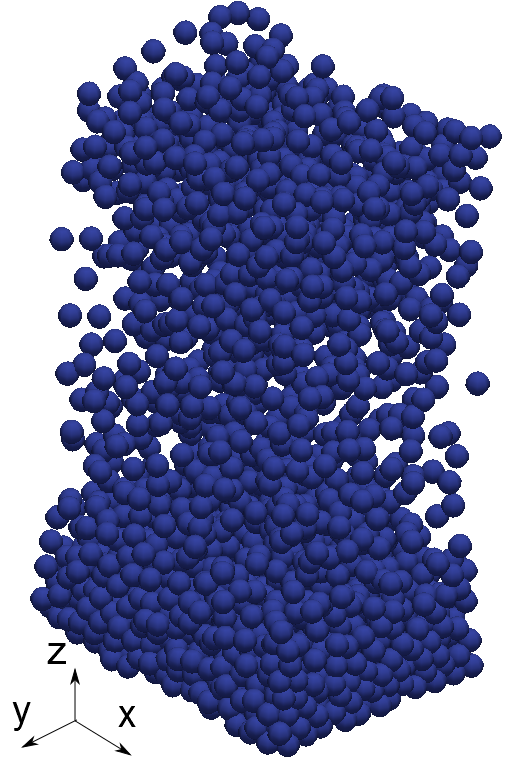
\includegraphics[width=\textwidth]{figures/fill01.png}
    \end{subfigure}
    \begin{subfigure}[b]{0.25\textwidth}
        \centering
        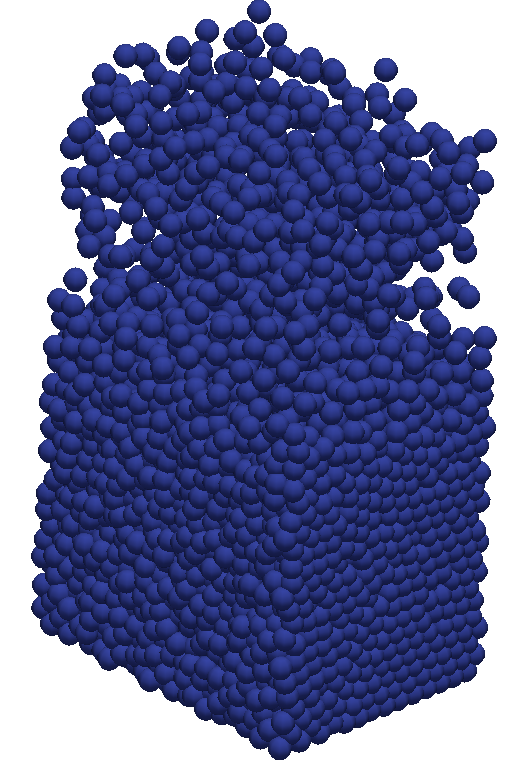
\includegraphics[width=\textwidth]{figures/fill02.png}
    \end{subfigure}
    \begin{subfigure}[b]{0.25\textwidth}
        \centering
        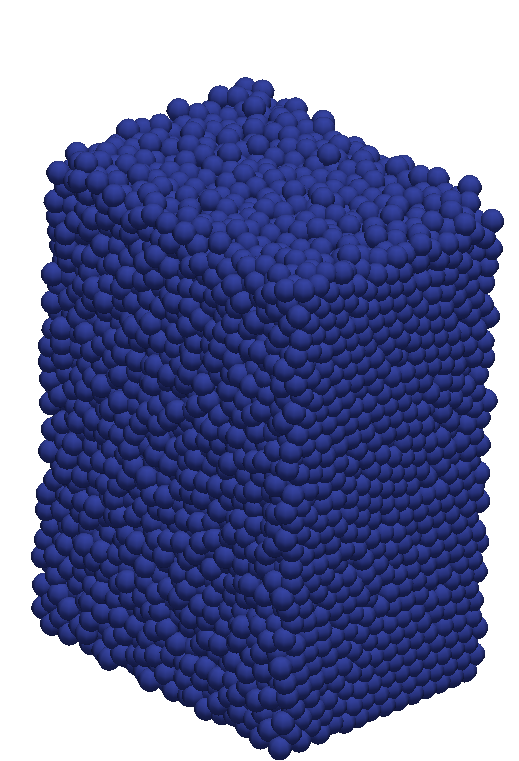
\includegraphics[width=\textwidth]{figures/fill03.png}
    \end{subfigure}
    \caption{Demonstrating the pouring process of pebbles into the control volume with at an early time (left), when it is nearly filled (middle) and after the pebbles have settled to negligible kinetic energy (right).}
\label{fig:fill01}
\end{figure}

The first attempt to pack the bed followed from the `recipes' we had used in physical experiments in the lab. That is, the pebbles were numerically poured into the volume from above and allowed to settle under their own weight (see \Cref{fig:fill01}), then the volume was vibrated while a roof was lowered to compact the system to $\phi = 0.64$, the desired packing fraction. This technique was ultimately abandoned in place of a less realistic but more computationally efficient technique which resulted in comparably packed beds.

In the preferred method, $N$ particles are inserted randomly, with large spacing, into a volume with an expanded $y$-direction. Gravity is not initialized and the coefficient of friction of the pebbles is set to $\mu = 0$. The system boundaries wrapped around the $y$-limits are slowly compressed until they reach the desired volume is obtained (as specified above). In the absence of friction, the pebbles move easily next to each other during the compression and there is no stored tangential forces when the pebble bed is `packed'. Next, the coefficient of friction is increased to a realistic level, $\mu = 0.2$, and gravity in the system is initialized. The bed is then allowed to come to rest, as measured by the kinetic energy of the system. At this point, the pebble bed is considered to be packed and the system state is saved, to be loaded into the heating routine.

%In this first study, we model pebble crushing without considering why the particular pebble should be cracking. In the model we randomly select pebbles from the ensemble, regardless of forces acting upon the pebble, and delete them entirely from the system. When a pebble is removed, the neighboring pebbles react due to the imbalance of forces, and the bed settles into a new configuration. 

To simulate the conditions of a solid breeder in a fusion reactor, where the heat is removed from the pebble bed \textit{via} contact to the containing structure, a constant temperature of $T_\text{c}$ is assigned to the vertical walls. Nuclear heating of the pebbles is simulated through a constant source term on each pebble. A representative heating rate of $Q_s = \frac{q_p'''}{\phi_0}$, where  $q_p'''= 8$ MW/m$^3$ and $\phi_0 = 0.64$.\cite{An20072233} The heating cycle runs until a thermal steady state is reached. Based on a measurement of the total thermal energy of the bed, $E_T =\sum_i^N m_iC_i T_i$, steady-state is determined as $\dt{E_T} = 0$ within a specified tolerance. Once at steady state, effective thermal conductivity of the beds is analyzed for comparison to experimental data on pebbles in vacuum.

Based on the boundary conditions of the system, the heat transfer becomes symmetric and one-dimensional in the $x$-direction from $x=0$ to the walls at $\frac{x}{d_p} = \pm 10$. The pebble bed has negligibly small variation of forces and temperatures in the $y$-direction due to the periodic boundary condition at the edges of the domain. Gravity effects are minor in the overall heat transfer and induce only a slight $z$-dependency to the results. Taking advantage of the pebble bed temperature profile's resemblance to a one-dimensional heat transfer problem to calculate an effective conductivity from an analytic, one-dimensional test case analogy.

Assuming a one-dimensional pebble bed, to find an effective conductivity, we step back into a continuum mechanics formulation where the pebble bed can be represented as a slab of solid material. We can analytically solve for the temperature equation in a slab with heat generation, symmetry about the centerline, and a constant boundary temperature condition.

At steady-state, the temperature of a material with constant temperature boundary conditions ($T(L) = T_s$), constant thermal conductivity ($\keff$), and nuclear heating ($q'''$) obeys the following equation

\begin{equation}\label{eq:continuum-heateqn}
    0 = \frac{\mathrm{d}^2T}{\mathrm{d}x^2} + \frac{q'''}{\keff}
\end{equation}

In nondimensional form, the temperature is
\begin{equation}
    \theta = \frac{T(x) - T_s}{T_0 - T_s}
\end{equation}
where $T_0$ is the temperature at the centerline of this slab (a value found momentarily). The length is nondimensionalized as
\begin{equation}
    x^* = \frac{x}{L}
\end{equation}

Thus \Cref{eq:continuum-heateqn} in nondimensional form is,
\begin{equation}\label{eq:continuum-heateqn-nondim}
    0 = \frac{\mathrm{d}^2\theta}{\mathrm{d}x^{*2}} + G
\end{equation}
where
\begin{equation}
    G = \frac{q'''L^2}{\keff(T_0 - T_s)}
\end{equation}

In the nondimensionalized form, the solution is revealed to be purely geometric,
\begin{equation}\label{eq:continuum-temperature-nondim}
    \theta = 1-x^{*2}
\end{equation}
as $T_0  - T_s = \frac{q'''L^2}{2\keff}$. The nondimensional temperature solution of \Cref{eq:continuum-temperature-nondim} is used to prove the one-dimensional assumption of heat transfer is justified for the pebble beds.


Noting that in this continuum mechanics formulation, we are assuming that the nuclear source, $q'''$ term is applied evenly over the entire volume. In our DEM formulation, our source term applies to a single pebble, $Q_s = \frac{q'''}{\phi}$.% To find the effective thermal conductivity of the `slab' of pebble bed, we must reconcile this discrepency. This is accomplished with the exchange of
% \begin{equation}\label{eq:q-source-translation}
%     q''' = \frac{Q_\text{tot}}{V_\text{tot}} = Q_s \phi_i
% \end{equation}
% where the pebble bed volume is given by the height, $H$, width, $W$, and length, $L$, and $Q_s$ is the source term on each pebble in the DEM ensemble. 

From the solution of \Cref{eq:continuum-heateqn-nondim}, we find the effective conductivity to be
\begin{equation}\label{eq:keff-formulation}
    \keff = \frac{q''' L^2}{2(T_0-T_s)}
\end{equation}

I use this formulation of \Cref{eq:continuum-heateqn-nondim} to analyze and compare the pebble beds.

For our representative pebble bed, after applying the nuclear heating and wall cooling, the steady-state temperature distributions of some representative volumes are given in \Cref{fig:init-packing-temp-dist}. Evident in all three pebble beds, though increasingly so for smaller packing fractions, are loose pebbles that have poor mechanical contact with neighboring pebbles and therefore have arbitrarily high temperatures (the magnitude is only limited by the time of the simulation). We refer to these pebbles as `rattlers'. The phenomena of hot rattlers is possible in DEM simulations because there is no other method of heat removal. This is a strong argument for the need to include helium purge gas in the thermal transport models of ceramic pebble beds. If these hot rattlers persist even in the presence of helium, it could lead to an unfavorable performance of the ceramic solid breeder -- the hot rattlers would sinter and prevent the outgassing of tritium, among other issues. The observation of these isolated pebbles is another motivator for the coupling of DEM to thermo-fluid models. In \Cref{fig:init-packing-temp-dist}, we also see that, intuitively, the more loosely packed the pebble bed, the higher the temperatures.


\begin{figure}[!ht]
    \centering
    \begin{subfigure}[b]{0.2\textwidth}
        \centering
        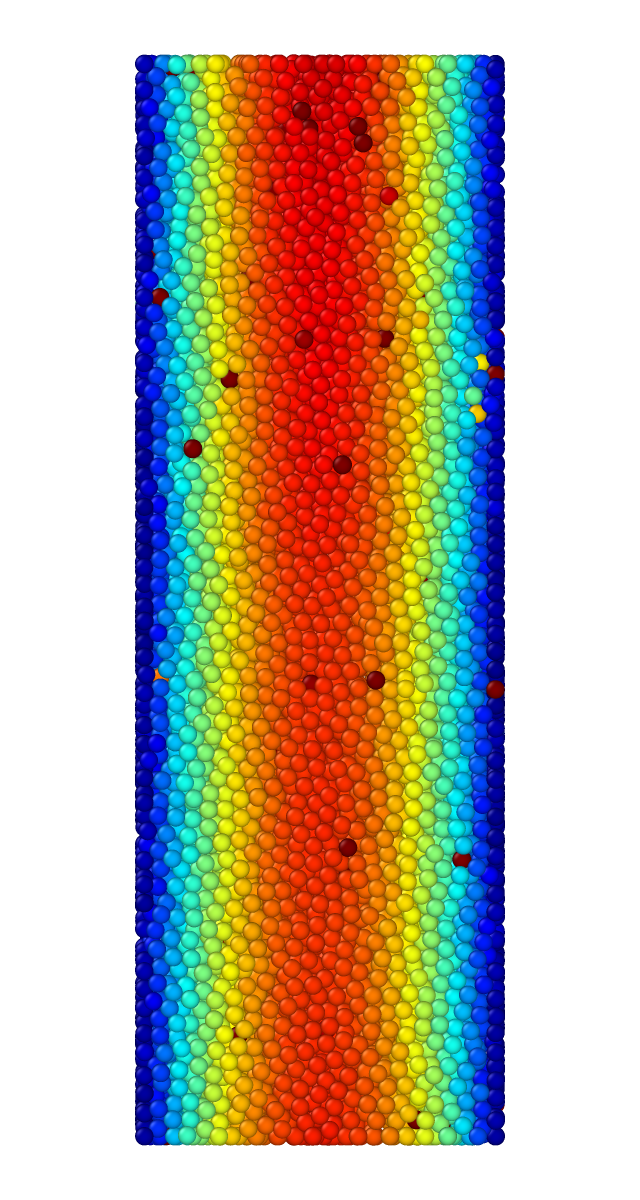
\includegraphics[width=\textwidth]{figures/initial_packing_study/61.png}
        \caption{$\phi_i = 61$\%}
    \end{subfigure}
    ~
    \begin{subfigure}[b]{0.2\textwidth}
        \centering
        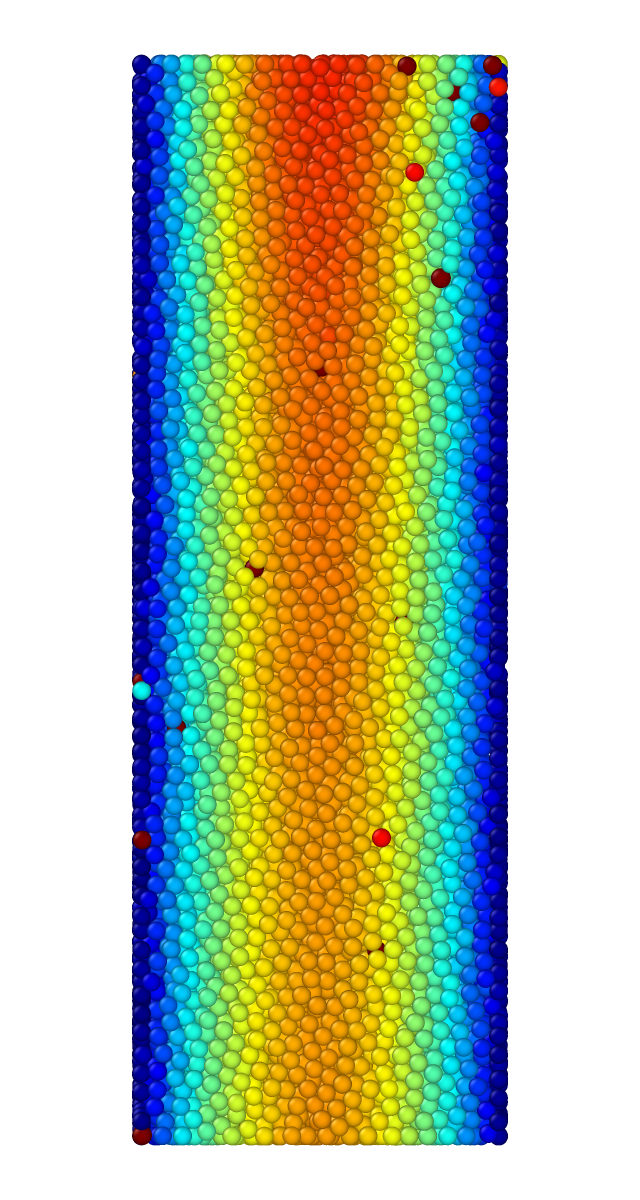
\includegraphics[width=\textwidth]{figures/initial_packing_study/62.png}
        \caption{$\phi_i = 62$\%}
    \end{subfigure}
    ~
    \begin{subfigure}[b]{0.2\textwidth}
        \centering
        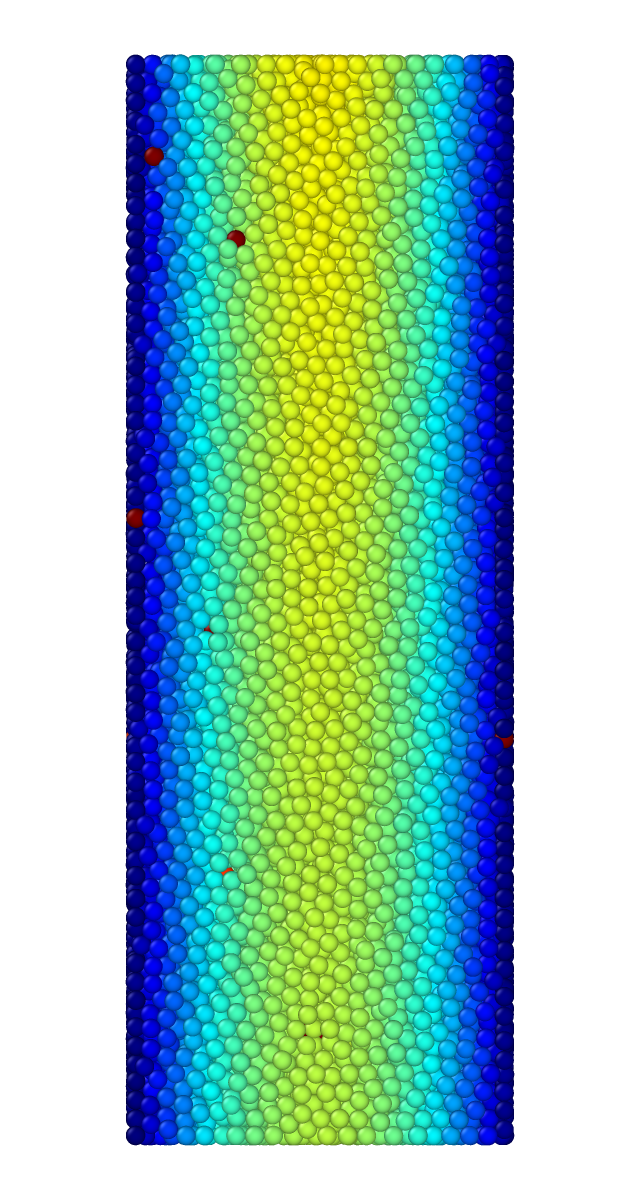
\includegraphics[width=\textwidth]{figures/initial_packing_study/64.png}
        \caption{$\phi_i = 64$\%}
    \end{subfigure}
    
    \begin{subfigure}[b]{0.3\textwidth}
        \centering
        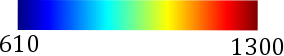
\includegraphics[width=\textwidth]{figures/initial_packing_study/colorbar.png}
    \end{subfigure}
\caption{Temperature distributions in representative packed beds with given initial packing fraction.}
\label{fig:init-packing-temp-dist}
\end{figure}

In order to calculate an effective conductivity of the pebble bed, we find an average temperature profile through the bed. Average values of the bed, along the $x$ direction, are generated \textit{via} averaging temperatures in bins. We create bins that are volumes slices of width $\Delta x$ that extend through the limits of the $y$- and $z$-directions. We then find the $n$ pebbles residing in the slices and take the mean value of their temperatures. The average, given by \Cref{eq:binned-T}, is also shown as the solid lines in \Cref{fig:keff-initial}. The binned average temperature is 
\begin{equation}\label{eq:binned-T}
    \langle T\rangle = \frac{1}{n}\sum_{i}^n T_i    
\end{equation}
Using the volume slices, average contact forces are also found, 
\begin{equation}\label{eq:binned-f}
    \langle F^{1/3} \rangle = \frac{1}{n}\sum_{i}^n F_{n,ij}^{1/3}
\end{equation}


Van Lew\etal~showed that the largest parameter governing the effective conductivity of a granular material like a packed bed is the magnitude of contact forces between pebbles.\cite{VanLew2014} In \Cref{fig:f-ave-initial}, we see the distribution of contact forces as scatter points. The binned average along $x$ is also plotted in the black line. \Cref{fig:f-scatter-59} is given as reference for a pebble bed for which the packing fraction does not completely fill the volume when the pebble bed quiesces. At $\phi_i = 59\%$ there are regions of gap between the top layer of pebbles and the container, as a result the contact forces are on the order of the accumulated weight of the pebbles in the volume. For packing fraction of $\phi_i = 61\%$, we have a relatively well-packed pebble bed with small average contact forces, $\langle F_n \rangle = \SI{5.9}{\newton}$. At an initial packing fraction of $\phi_i = 64\%$, \textit{for the geometry of this bed}, we see somewhat larger average contact forces, $\langle F_n \rangle = \SI{25.9}{\newton}$. In large-volume experiments on pebble beds, such a large contact force would be indicative of being under slight compression and, as such, we expect the effective thermal conductivity of the bed to be larger than the well-packed case of $\phi_i = 61\%$. The effective thermal conductivities are given in the temperature plots of \Cref{fig:keff-initial}.

\begin{figure}[!ht]
    \centering
    \begin{subfigure}[b]{0.45\textwidth}
        \centering
        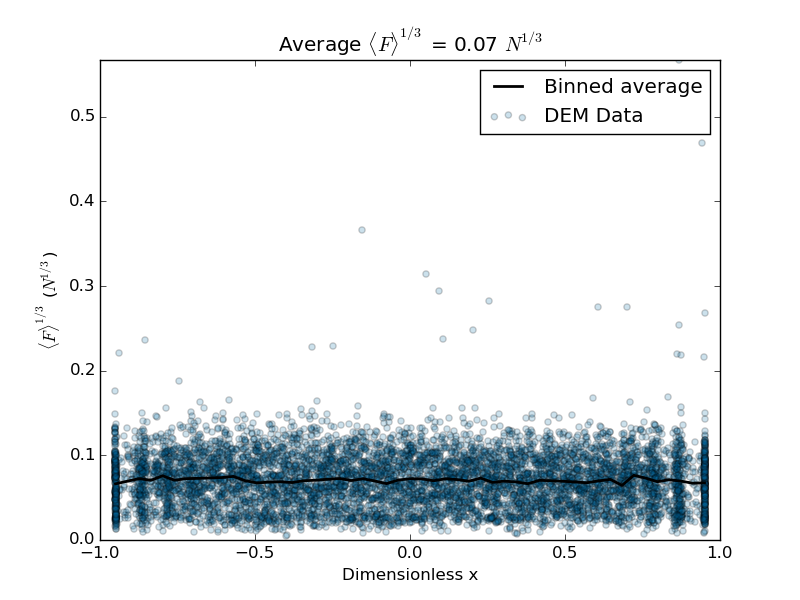
\includegraphics[width=\textwidth]{figures/initial_packing_study/f-scatter-59.png}
        \caption{$\phi_i = 59\%$}\label{fig:f-scatter-59}
    \end{subfigure}
    ~
    \begin{subfigure}[b]{0.45\textwidth}
        \centering
        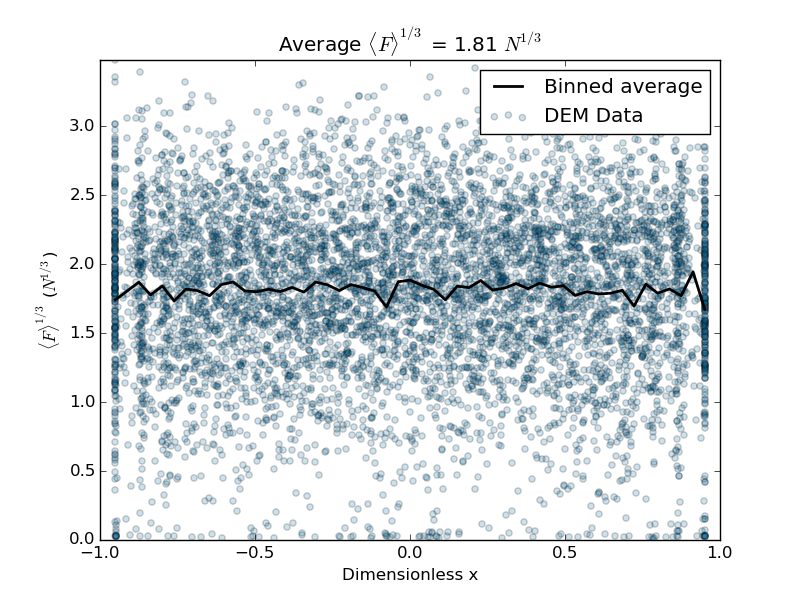
\includegraphics[width=\textwidth]{figures/initial_packing_study/f-scatter-61.png}
        \caption{$\phi_i = 61\%$}
    \end{subfigure}
    
    \begin{subfigure}[b]{0.45\textwidth}
        \centering
        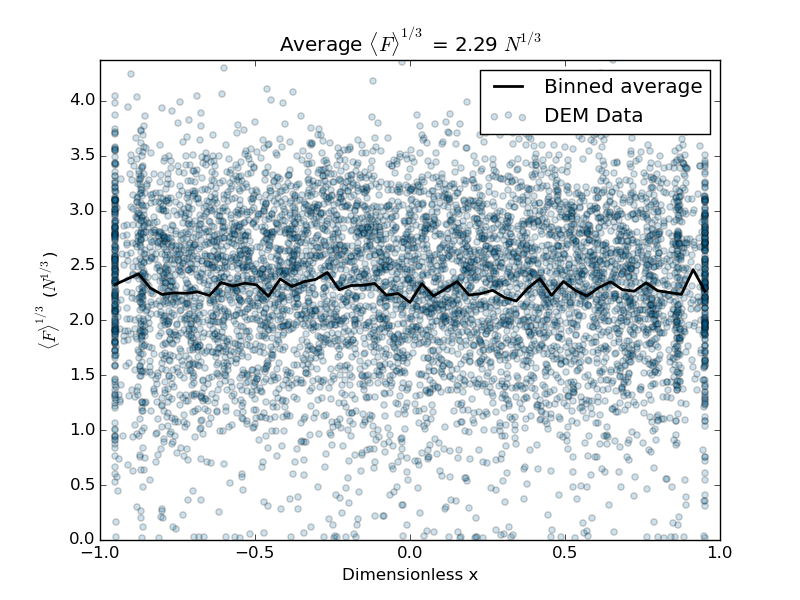
\includegraphics[width=\textwidth]{figures/initial_packing_study/f-scatter-62.png}
        \caption{$\phi_i = 62\%$}
    \end{subfigure}
    ~
    \begin{subfigure}[b]{0.45\textwidth}
        \centering
        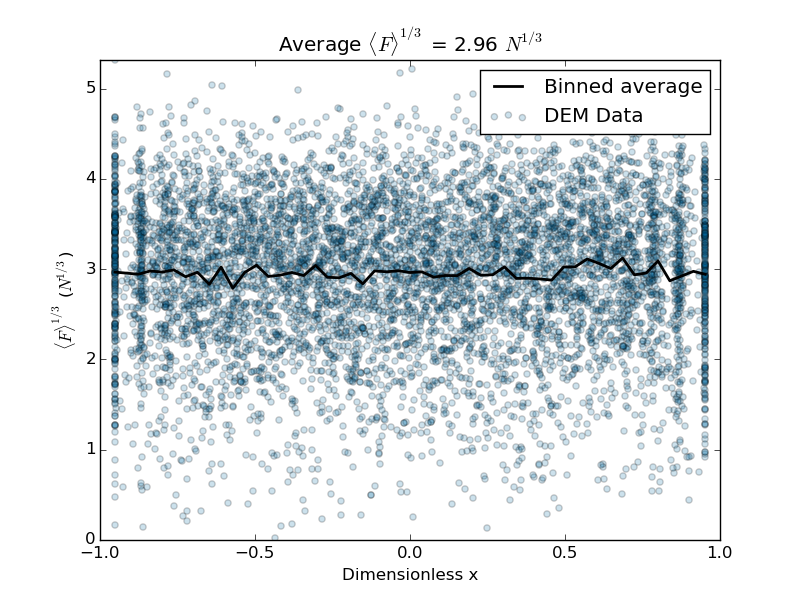
\includegraphics[width=\textwidth]{figures/initial_packing_study/f-scatter-64.png}
        \caption{$\phi_i = 64\%$}
    \end{subfigure}
    \caption{Contact forces in the initially packed beds .}
\label{fig:f-ave-initial}
\end{figure}

\begin{figure}[!ht]
    \centering
    \begin{subfigure}[b]{0.45\textwidth}
        \centering
        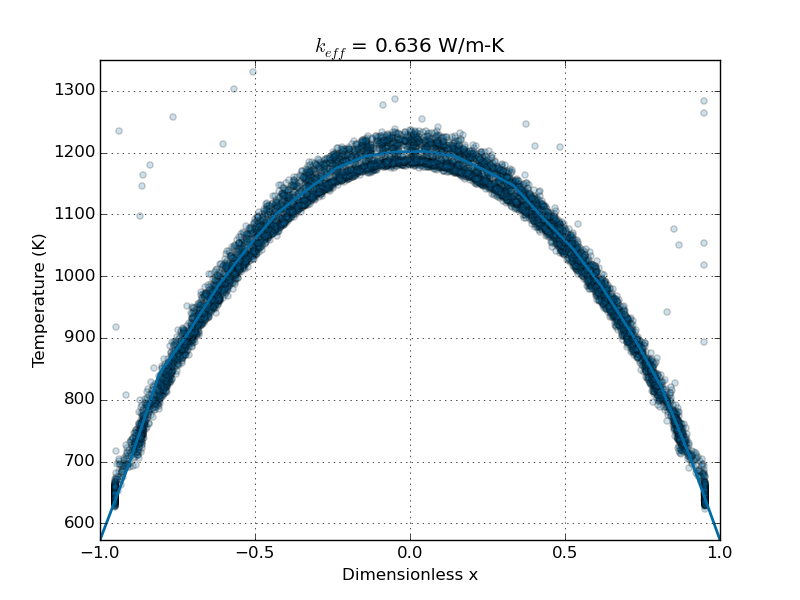
\includegraphics[width=\textwidth]{figures/initial_packing_study/keff-61.png}
        \caption{$\phi_i = 61\%$}
    \end{subfigure}
    ~
    \begin{subfigure}[b]{0.45\textwidth}
        \centering
        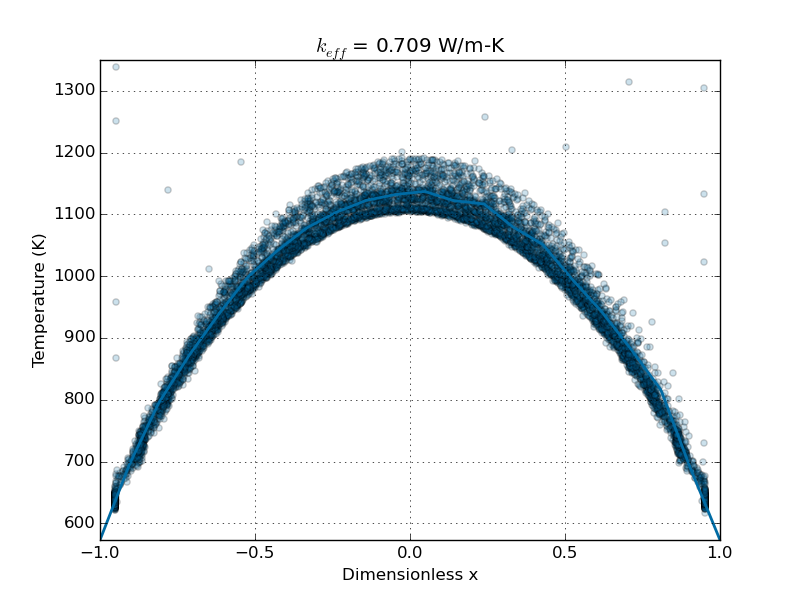
\includegraphics[width=\textwidth]{figures/initial_packing_study/keff-62.png}
        \caption{$\phi_i = 62\%$}
    \end{subfigure}

    \begin{subfigure}[b]{0.45\textwidth}
        \centering
        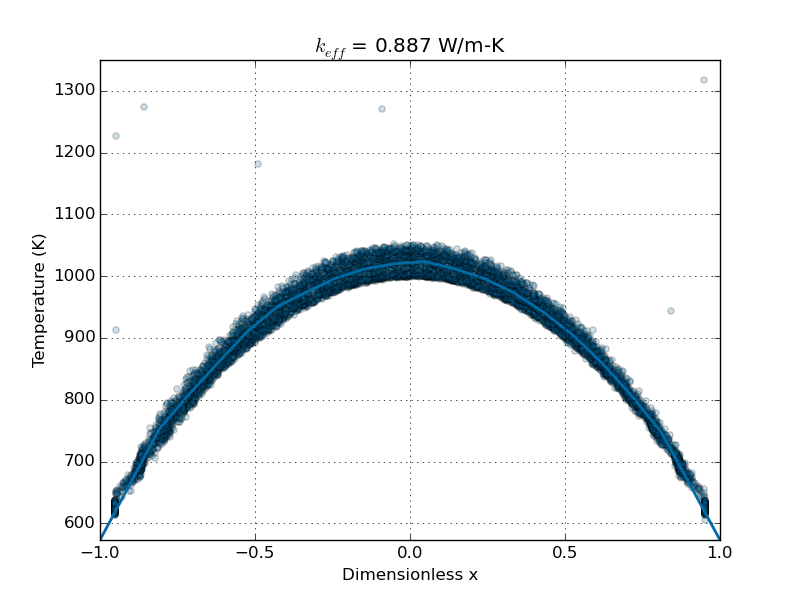
\includegraphics[width=\textwidth]{figures/initial_packing_study/keff-64.png}
        \caption{$\phi_i = 64\%$}
    \end{subfigure}
    \caption{$\keff$ for the packed beds is higher than values measured in experiments in vacuum.}
\label{fig:keff-initial}
\end{figure}

From \Cref{fig:keff-initial}, we see that even the most compliant well-packed bed of case $\phi_i = 0.61$, the effective thermal conductivity is more than three times larger than the measured effective conductivity from experimental data.\cite{ENOEDA} We will see that part of this discrepency is due the current model not accounting for surface roughness of pebble material. For the simulations generating the data of \Cref{fig:keff-initial}, the smooth particle contact conductance model of Batchelor \& O'Brien was used (see \Cref{eq:cheng-modification-batchelor}). In experimental measurements of effective thermal conductivity with roughness, at small loads, effective thermal conductivity of face-centered cubic steel spheroids in an air environment reduced approximately 25\% between cases between a smooth surface ($\sigma = $ \SI{0.03}{\micro\meter}) and rough ($\sigma = $ \SI{1.7}{\micro\meter}).\cite{Buonanno2003a} In spite of the lack of data for roughness of the specific pebbles used in the experiments of Enoeda\etal, we will see that including surface roughness, \textit{via} \Cref{eq:micro-macro-conductance}, allows our DEM models to obtain comparable effective thermal conductivities.

Following ranges of values found in a variety of experimental data,\cite{Bahrami2004} we can choose average parameters for roughness. The asperity height, ranging in experiments from \SIrange{0.12}{13.94}{\micro\meter}; we use an average value of $\sigma = \SI{5}{\micro\meter}$. Vickers hardness is reported for \lit~as $H = 363(1-2.36 \epsilon)$~\si{\mega\pascal}, where $0.1 \le \epsilon \le 0.3$ is the porosity of the bulk ceramic; with $\epsilon = 0.2$, $H = \SI{192}{\mega\pascal}$.\cite{Gierszewski1998,Roux1996a} However, it is unclear if the reported value is the microhardness or macrohardness (as defined by ASTM E384). Surface microhardness can be much larger than bulk hardness.\cite{Bahrami20063691} Regardless, for this study we set the microhardness value equal to $H = \SI{192}{\mega\pascal}$. No Vickers hardness data has been reported for \lis. Using the place-holder roughness values, we use \Cref{eq:micro-macro-conductance} form of conductance to run the above cases again.

Before discussing the results of effective thermal conductivity with roughness, we analyze the effect of the above roughness parameters in order to have an understanding of what to expect in packed beds with rough-surface pebbles. We normalize the heat conductance of \Cref{eq:micro-macro-conductance} by the smooth-sphere conductance of \Cref{eq:cheng-modification-batchelor},
\begin{equation}\label{eq:hjoverhc}
\Gamma = \frac{H_j}{H_c} = \frac{\frac{1}{2k^*a}}{\left(\frac{H'}{E^*\delta_n}\right)^{0.96}\frac{0.031\sigma^{0.598}}{1.720k^*a^{1.04}} + \frac{1}{2k^*a}}
\end{equation}


Therefore we see from \Cref{eq:hjoverhc} that $\Gamma$ is a quantification of reduction in heat conductance due to roughness parameters. Using the a hardness of $H = \SI{15}{\giga\pascal}$, we then find heat conductance reduction, $\Gamma$ as a function of contact force (which determines the value of $a$) and asperity height, $\sigma$. The contour of $\Gamma$ is given in \Cref{fig:roughness-parameters}.

\begin{figure}[ht]
\centering
    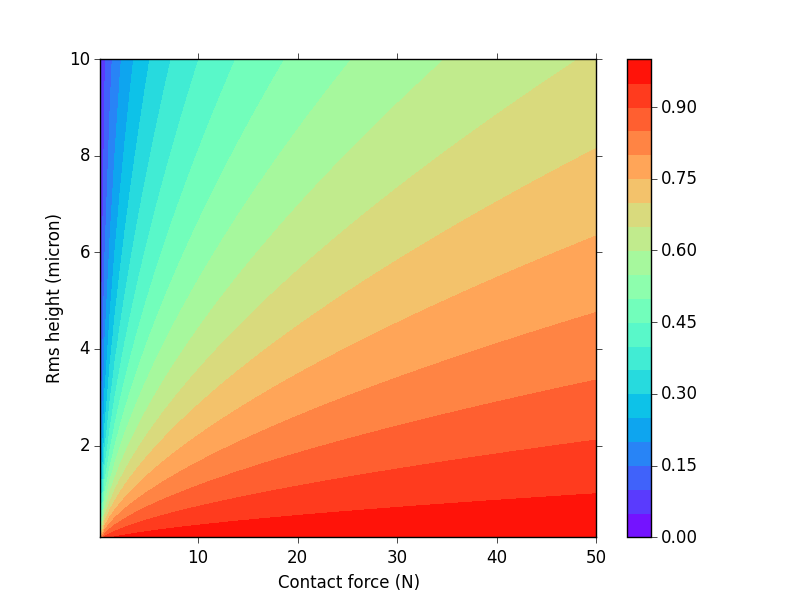
\includegraphics[width=\singleimagewidth]{figures/conductance-contour-roughness.png}
    \caption{Colorbar gives value of $\Gamma$, the measure of reduction in heat conductance comparing calculations with roughness and smooth sphere approximations.}
    \label{fig:roughness-parameters}
\end{figure}

The bed initially packed to $\phi_i = 0.64$, had average contact forces of about \SI{25}{\newton}. According to \Cref{fig:roughness-parameters}, at that force level, with an asperity of \SI{5}{\micro\meter}, contact heat conductance of a rough pebble is 75\% of a similar contact between smooth pebbles. The bed packed to $\phi_i = 0.61$ had average contact forces of \SI{5.9}{\newton}; in this case heat conductance has been reduced approximately 45\% from the smooth approximation. The total effective thermal conductivity is the macroscopic result of heat conductance between all pebbles and can not be linearly extrapolated from heat conductance of any single contact, nonetheless, the measure of $\Gamma$ provides insight into approximate scales of reduction in effective thermal conductivity we should expect when roughness is taken into account.  


Temperature distributions in pebble beds with roughness, along with measures of effective thermal conductivity are given in \Cref{fig:keff-rough-initial}. Accounting for roughness of the pebbles in contact, the effective thermal conductivity of numeric pebble beds approaches the value found in experimental studies of pebble beds in vacuum. When the initial packing fraction is $\phi_i = 0.61$, the effective thermal conductivity falls to $\keff = \SI{0.398}{\watt\per\meter\per\kelvin}$, which compares quite well to experimental measurement of $\keff = \SI{0.2}{\watt\per\meter\per\kelvin}$.


\begin{figure}[ht]
    \centering
    \begin{subfigure}[b]{0.45\textwidth}
        \centering
        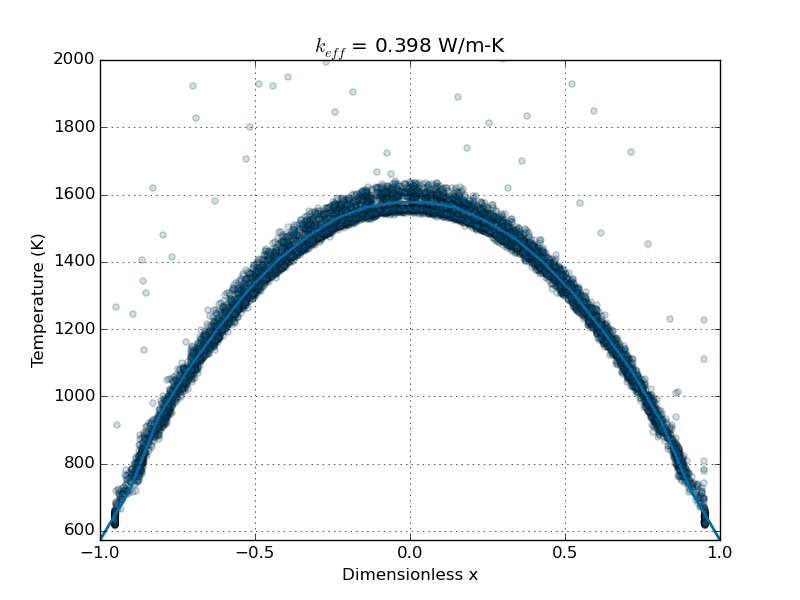
\includegraphics[width=\textwidth]{figures/initial_packing_study/keff-rough-61.png}
        \caption{$\phi_i = 61\%$}
    \end{subfigure}
    ~
    \begin{subfigure}[b]{0.45\textwidth}
        \centering
        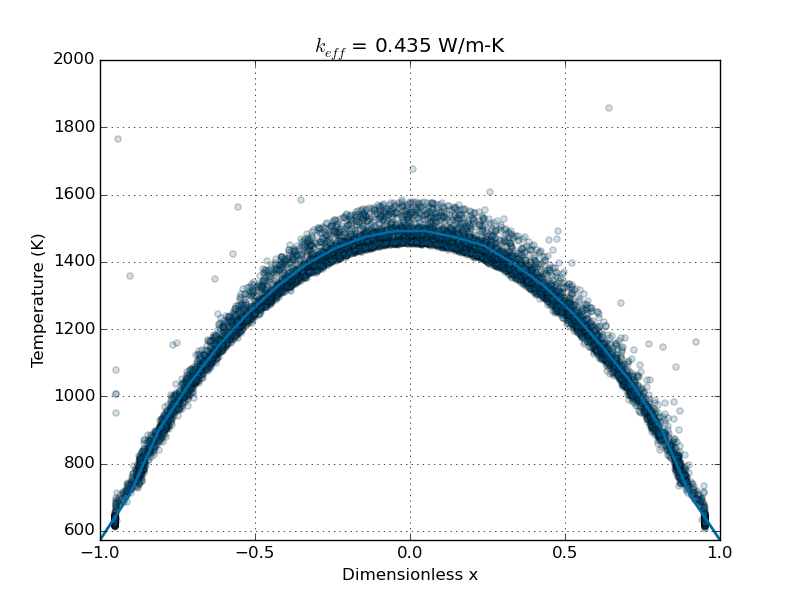
\includegraphics[width=\textwidth]{figures/initial_packing_study/keff-rough-62.png}
        \caption{$\phi_i = 62\%$}
    \end{subfigure}

    \begin{subfigure}[b]{0.45\textwidth}
        \centering
        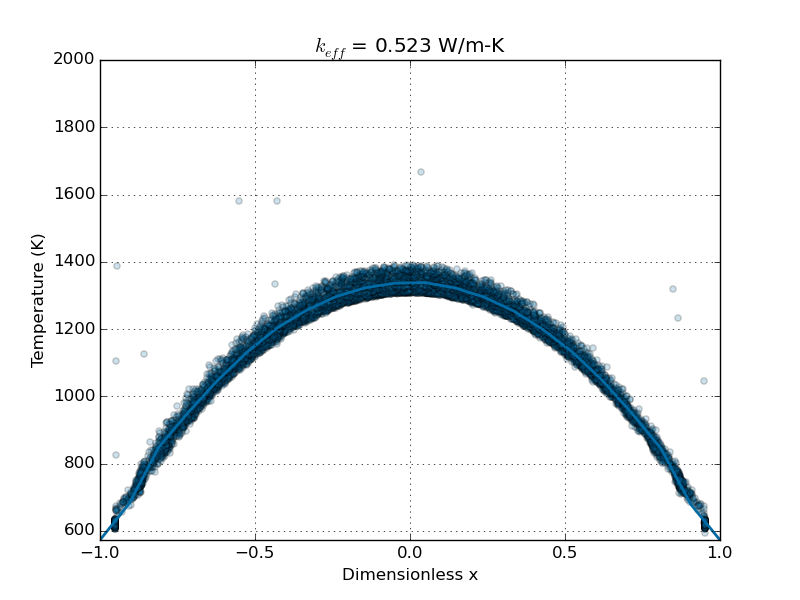
\includegraphics[width=\textwidth]{figures/initial_packing_study/keff-rough-64.png}
        \caption{$\phi_i = 64\%$}
    \end{subfigure}
    \caption{$\keff$ with roughness for given initial packing fractions. Reduced initial packing fractions had lower initial contact forces and therefore effective conductivity values closer to experimentally measured ones.}
\label{fig:keff-rough-initial}
\end{figure}

\FloatBarrier

The effective conductivities of models with the smooth-sphere and roughness approximations are plotted together in \Cref{fig:keff-vacuum-comparisons}. For reference, the grey bar indicates the window of experimental measurements for effective conductivity in vacuum.

\begin{figure}[ht]
\centering
    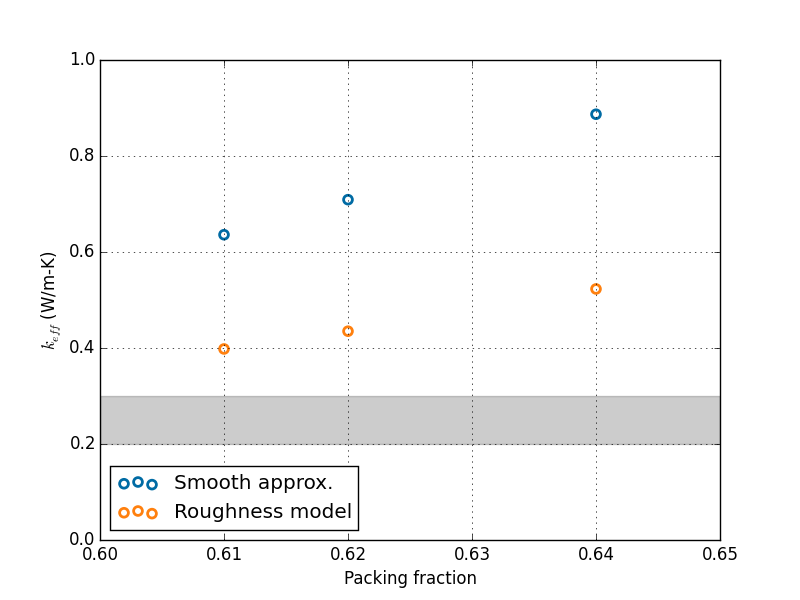
\includegraphics[width=\singleimagewidth]{figures/initial_packing_study/keff-comparisons.png}
    \caption{Comparison of effective conductivity measurements for \lit.}
    \label{fig:keff-vacuum-comparisons}
\end{figure}

The combination of microhardness and asperity height resulted in substantial drops in the effective thermal conductivity of these representative pebble beds. The reductions in effective conductivity were 37\%, 39\%, and 41\% for initial packing fractions of 61\%, 62\%, and 64\%, respectively. While these reductions make the effective conductivity calculated with DEM approach the experimental measurements for pebble beds in vacuum, the values are still more than 25\% higher. The Vicker's microhardness value used in this study could be measured again for other production techniques of lithium ceramics and variations in that value could lead to DEM results that approach even closer to experimental values. Moreover, the arbitrarily-chosen rms asperity height needs to be measured for ceramic pebbles for more accurate roughness contact resistance modeling. Lastly, the majority of ceramic pebbles produced for solid breeders have non-perfect sphericity, some are ovoid or ellipsoidal. However, in the current implementation of DEM, the pebbles are all perfectly spherical. The impact on effective thermal conductivity with geometric variations of the packing material is fertile grounds for future studies.




%%%%%%%%%%%%%%%%%%%%%%%%%%%%%%%%%%%%%%%%%%%%%%%%%%%%%%%%%%%%%%%%%%%%%%%%%%%%%%%%%%%%%%%%%%%%%%%%%%%%%%%%%%%%
%%%%%%%%%%%%%%%%%%%%%%%%%%%%%%%%%%%%%%%%%%%%%%%%%%%%%%%%%%%%%%%%%%%%%%%%%%%%%%%%%%%%%%%%%%%%%%%%%%%%%%%%%%%%
%
% new section
%
%%%%%%%%%%%%%%%%%%%%%%%%%%%%%%%%%%%%%%%%%%%%%%%%%%%%%%%%%%%%%%%%%%%%%%%%%%%%%%%%%%%%%%%%%%%%%%%%%%%%%%%%%%%%
%%%%%%%%%%%%%%%%%%%%%%%%%%%%%%%%%%%%%%%%%%%%%%%%%%%%%%%%%%%%%%%%%%%%%%%%%%%%%%%%%%%%%%%%%%%%%%%%%%%%%%%%%%%%
\section{Elastic Modulus Implementation in DEM for Ceramic Pebbles}\label{sec:exp-reduction-factor}
The discrete element method has been used by many ceramic breeder researchers to model the interaction of individual pebbles in an ensemble.\cite{An20071393, Lu2000, Zhao2010, Gan:2010uq, Annabattula2012a, VanLew2014} In the past studies, the elastic modulus of the ceramic materials used in DEM simulations was taken from historical data, for instance lithium metatitanate from Ref.~\cite{Gierszewski1998}. Furthermore, the assumption of Hertzian descriptions of normal contact for the pebbles is also assumed to be true without direct validation. In our experimental test stand for crushing individual pebbles, shown in \Cref{fig:nfri-fmax}, our equipment was able to record accurate measurements of the force-travel relationship for each pebble. Using the data, we will directly test the validity of Hertzian contact laws for describing interactions of lithium ceramics. 

\begin{figure}[ht]
        \centering
        \begin{subfigure}[b]{\doubleimagewidth}
                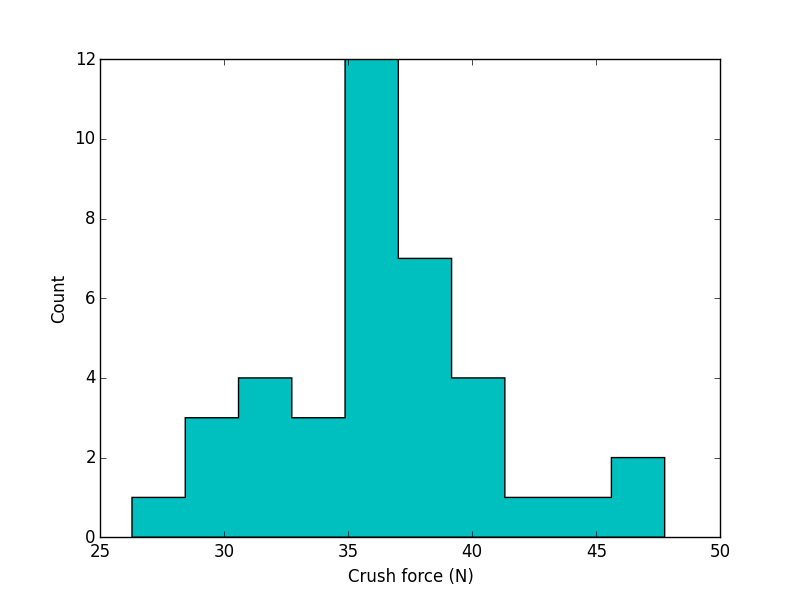
\includegraphics[width=\textwidth]{figures/nfri-1mm-fmax-histogram.png}
                \caption{$\bar{d}_p = 1$ mm}
                \label{fig:nfri-1-exp-fmax}
        \end{subfigure}
        ~
        \begin{subfigure}[b]{\doubleimagewidth}
                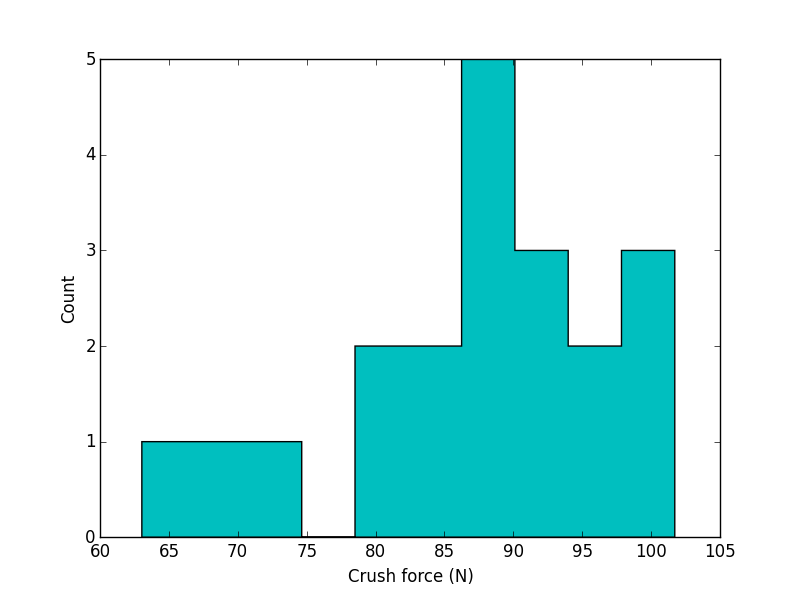
\includegraphics[width=\textwidth]{figures/nfri-1.5mm-fmax-histogram.png}
                \caption{$\bar{d}_p = 1.5$ mm}
                \label{fig:nfri-1.5-exp-fmax}
        \end{subfigure}
        \caption{Crush forces of \lit~pebbles display probability distributions around mean values for each average diameter batch.}\label{fig:nfri-fmax}
\end{figure}

The derivation of the Hertz force can be found on page~\pageref{eq:hertz-normal-force}. The result is given again here for reference:
\begin{equation*}
  F_{n,ij} = \frac{4}{3}E_{ij}^* \sqrt{R_{ij}^*} \, \delta_{n,ij}^{3/2}
\end{equation*}
and, again, the pair elastic modulus and radius are
\begin{align*}
\frac{1}{E^*} & = \frac{1-\nu_i^2}{E_i} + \frac{1-\nu_j^2}{E_j} \\
\frac{1}{R^*} & = \frac{1}{R_i} + \frac{1}{R_j}
\end{align*}

In experiments where we press a ceramic pebble between two anvils, we measure the travel, $s$, of the crosshead rather than the pebble overlap. We modify \Cref{eq:hertz-normal-force} to be represented in terms of travel ($s = 2\delta$). Furthermore, for a pebble ($R_i = R_p$) in contact with a smooth plane ($R_j \rightarrow \infty$), the relative radius is simply $R^* = R_p = d_p/2$. We write the elastic modulus of the pebble as $E_p$ and for the test stand's anvil as $E_s$; similarly for the Poisson ratios of the two materials. The Hertz force acting upon a pebble between anvils is then expressed as a function of the pebble and anvil properties as,
\begin{equation}\label{eq:contact-force}
        F = \left[\frac{1}{3}\frac{\sqrt{d_p}}{\frac{1-\nu_p^2}{E_p} + \frac{1-\nu_s^2}{E_s}}\right] s^{3/2}
\end{equation}

The elastic modulus and Poisson ratio of the test stand are known values that do not vary between pebble experiments. Similarly, in the application of Hertz theory, we also assume the elastic modulus and Poisson ratio of the ceramic are also known and constant. In that case, \textit{for any given pebble diameter}, the term inside the bracket ought to be composed entirely of constants for any given pebble; there would therefore be a single force-travel response possible -- based only on $s$. Using material properties given in Ref.~\cite{Gierszewski1998} for \lit, we plot a set of parametric curves based on diameter over a range of travel. The properties we have used for the nickel-alloy anvil of our test stand and \lit~are given in \Cref{tab:hertz-dp-study-props}. The curves are given in \Cref{fig:hertz-dp-dependence}.

\begin {table}[ht] %
\caption{Material properties used for \lit~and nickel-alloy platen}
\label {tab:hertz-dp-study-props} \centering %
\begin {tabular}{ cccccc }
\toprule %
$E_\text{peb}$      &     $\nu_\text{peb}$  &   $E_\text{stand}$        &     $\nu_\text{stand}$    \\
(GPa)           &                   &   (GPa)               &                   \\\toprule
126             &   0.24                &   220                 &   0.27                \\\bottomrule
\end{tabular}
\end{table}

\begin{figure}[ht]
	\centering
	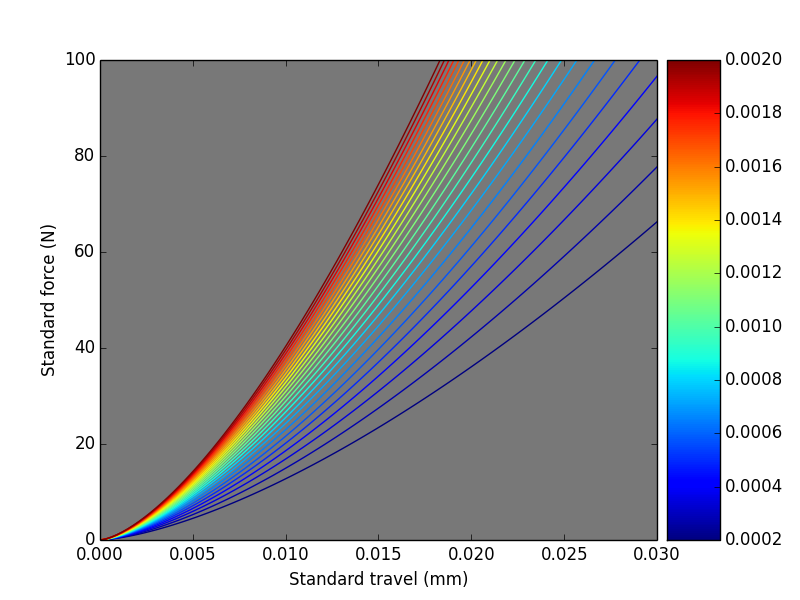
\includegraphics[width = \singleimagewidth]{figures/hertz-dp-dependence}
	\caption{Hertzian responses of \lit~pebbles compressed between platens. The colormap shows pebble diameters in \si{m}. The diameters span an order of magnitude from $d_p = \SI{0.2}{\milli\meter}$ to $d_p = \SI{2}{\milli\meter}$.}\label{fig:hertz-dp-dependence}
\end{figure}

\Cref{fig:hertz-dp-dependence} shows that, for a given pebble, that is strictly obeying Hertz theory, there is only a single force-displacement curve it can follow. However, during our experiments on \lit~pebbles, we observed behavior such as the curves shown in \Cref{fig:nfri-exp-curves}. The diameters of the pebbles are mapped to the colormap on the right side of the figures. These pebbles are responding much different than the expected Hertzian curve, predicted by \Cref{eq:contact-force}. 

We can confirm that the force-travel relationship goes as $F\propto s^{3/2}$ by plotting the force-travel data on log-log plots; the slope of the data represents the power relationship of force and travel. The log-log plots are given in \Cref{fig:nfri-exp-curves-loglog}. The slope of the response is calculated for each experimental curve and a histogram is collected in \Cref{fig:nfri-loglog-slopes}. For both sets of \lit~pebbles, the data is heavily centered around a slope of $n=1.5$, validating the dependence of force on travel as fitting Hertzian predictions.

\begin{figure}[ht]
        \centering
        \begin{subfigure}[b]{\doubleimagewidth}
                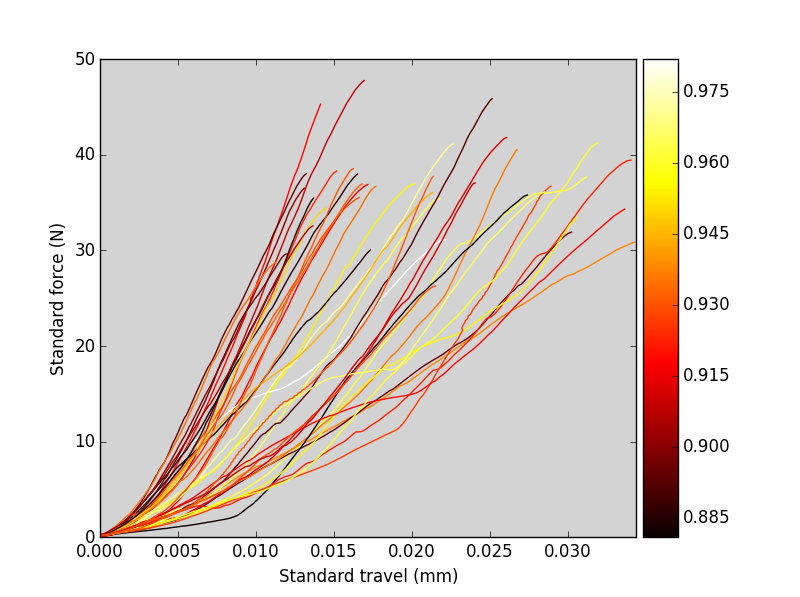
\includegraphics[width=\textwidth]{figures/nfri-1mm-data.png}
                \caption{$\bar{d}_p = 1$ mm}
                \label{fig:nfri-1-exp-colormap}
        \end{subfigure}
        ~
        \begin{subfigure}[b]{\doubleimagewidth}
                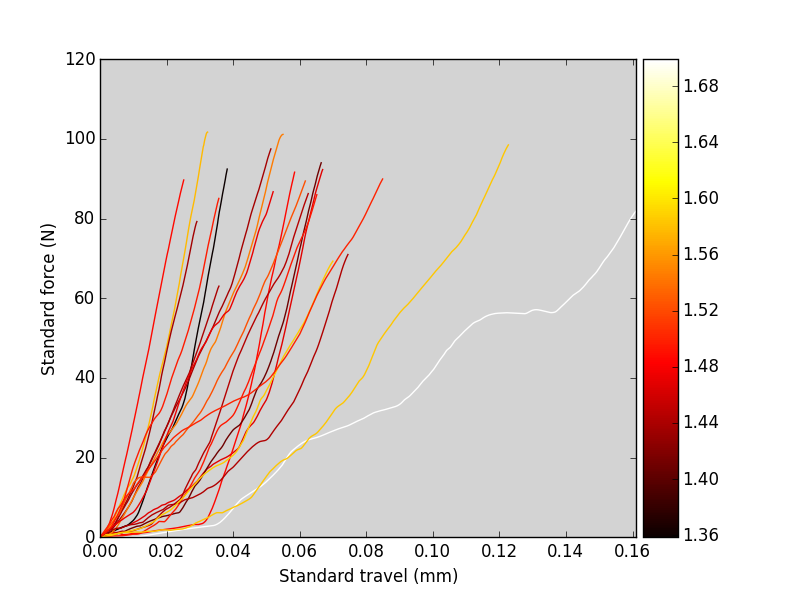
\includegraphics[width=\textwidth]{figures/nfri-1.5mm-data.png}
                \caption{$\bar{d}_p = 1.5$ mm}
                \label{fig:nfri-1.5-exp-colormap}
        \end{subfigure}
        \caption{Experimental measurements of pebble force as a function of cross-head travel.}\label{fig:nfri-exp-curves}
\end{figure}

\begin{figure}[ht]
        \centering
        \begin{subfigure}[b]{\doubleimagewidth}
                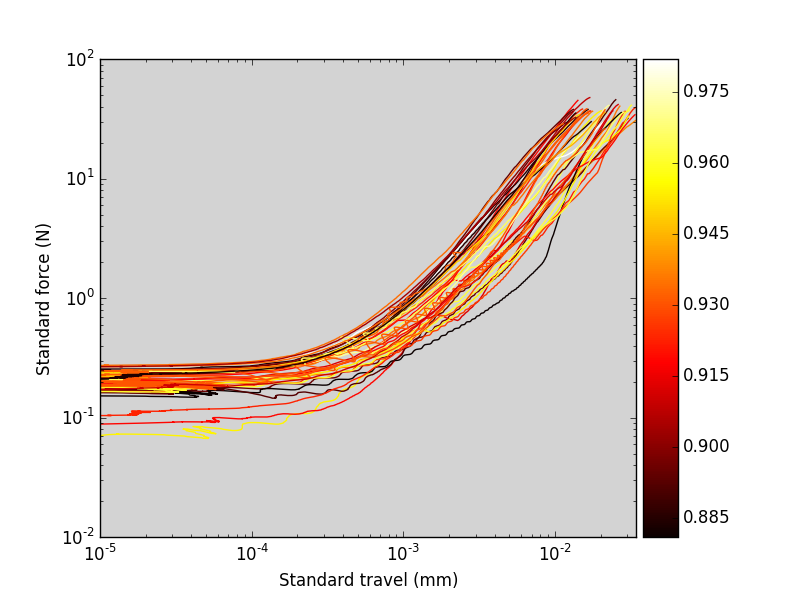
\includegraphics[width=\textwidth]{figures/nfri-1mm-data-loglog.png}
                \caption{$\bar{d}_p = 1$ mm}
                \label{fig:nfri-1-exp-loglog}
        \end{subfigure}
        ~
        \begin{subfigure}[b]{\doubleimagewidth}
                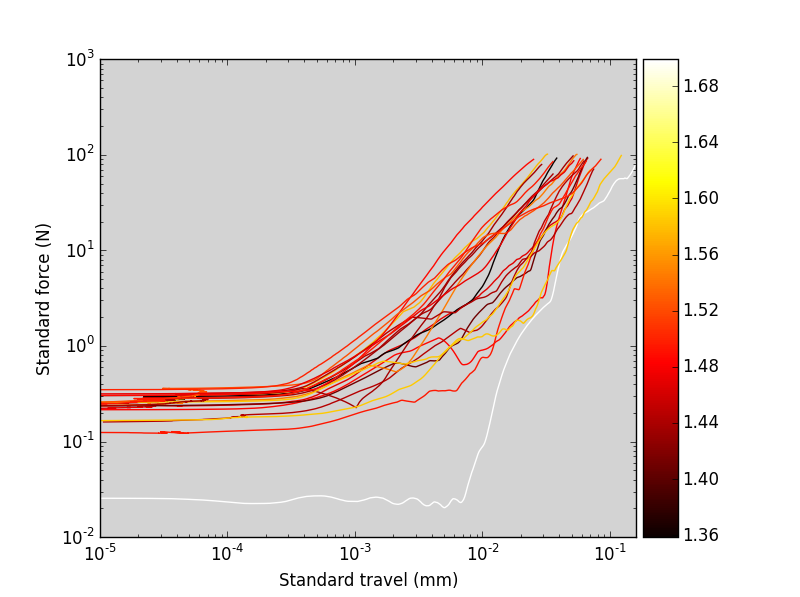
\includegraphics[width=\textwidth]{figures/nfri-1.5mm-data-loglog.png}
                \caption{$\bar{d}_p = 1.5$ mm}
                \label{fig:nfri-1.5-exp-loglog}
        \end{subfigure}
        \caption{Log-log plots of experimental measurements of pebble force as a function of cross-head travel.}\label{fig:nfri-exp-curves-loglog}
\end{figure}

\begin{figure}[ht]
        \centering
        \begin{subfigure}[b]{\doubleimagewidth}
                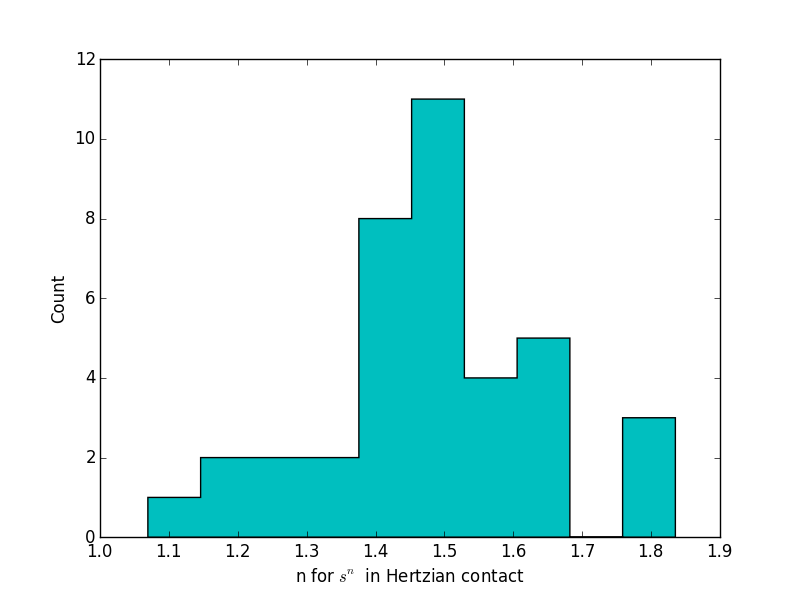
\includegraphics[width=\textwidth]{figures/nfri-1mm-loglog-slope.png}
                \caption{$\bar{d}_p = 1$ mm}
                \label{fig:nfri-1-exp-slope}
        \end{subfigure}
        ~
        \begin{subfigure}[b]{\doubleimagewidth}
                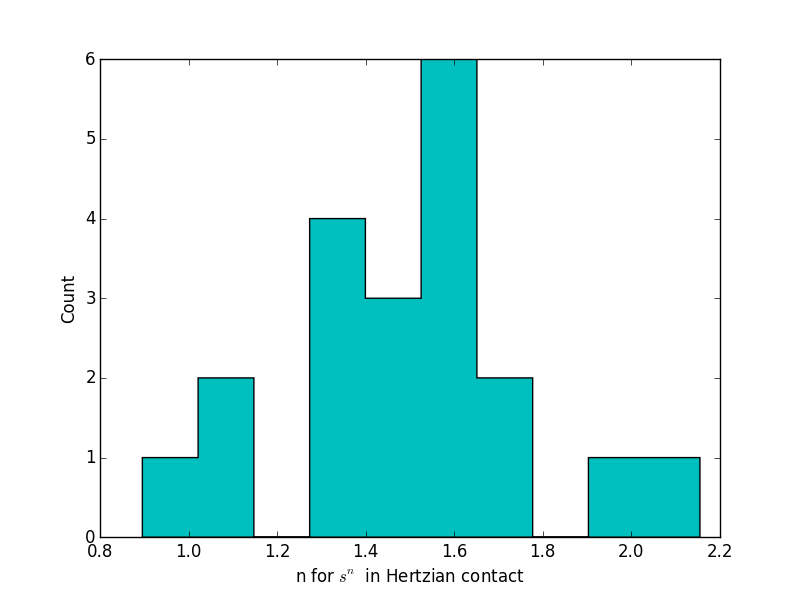
\includegraphics[width=\textwidth]{figures/nfri-1.5mm-loglog-slope.png}
                \caption{$\bar{d}_p = 1.5$ mm}
                \label{fig:nfri-1.5-exp-slope}
        \end{subfigure}
        \caption{Slopes from the log-log plots of experimental measurements of pebble force as a function of cross-head travel show the relation is approximately $F\propto s^{1.5}$.}\label{fig:nfri-loglog-slopes}
\end{figure}

We propose the experimental curves of force travel can be explained \textit{via} unique reductions in elastic modulus of each pebble. We introduce an `apparent' elastic modulus for each pebble which is iteratively found as the elastic modulus which provides the best fit when used in \Cref{eq:contact-force} and compared to force-travel responses from experiments. The apparent elastic modulus is reported normalized against the \lit~elastic modulus from literature, $E_\text{lit}$, 
\begin{equation}
	\kappa = \frac{E_\text{peb}}{E_\text{lit}}
\end{equation}
where we introduce $\kappa$ as a softening coefficient. The sintered pebble value of elastic modulus for \lit~is taken from Ref.\cite{gnielinski1982berechnung} to be $E_\text{lit}= \si{124~GPa}$. Iterating over apparent elastic modulus, the L2-norm of the difference between Hertzian and experimental curves is used as the `error'. The L2 norm, $A$ for a given array, $a$ is 
\begin{equation}
	||A||_F = \left[\sum_{i,j}\textrm{abs}(a_{i,j})^2\right]^{1/2}
\end{equation}

This is a convenient way to compare the error at every point along the force-displacement curves. When the error is minimized, the apparent elastic modulus is recorded and a softening coefficient is calculated. A Hertzian curve (in black), using the apparent elastic modulus in \Cref{eq:contact-force}, is plotted alongside its respective experimental curve in \Cref{fig:nfri-exp-hertz}

\begin{figure}
        \centering
        \begin{subfigure}[b]{\doubleimagewidth}
                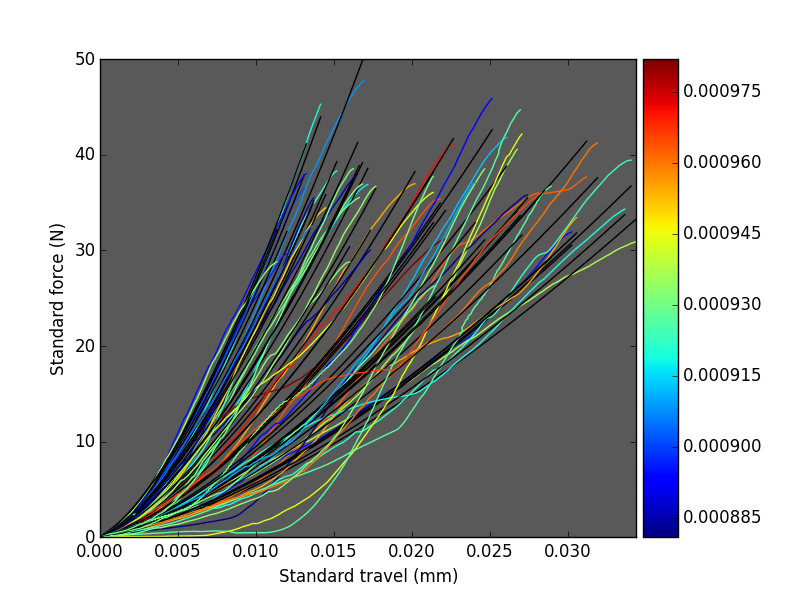
\includegraphics[width=\textwidth]{figures/nfri-1mm-hertz-colormap.png}
                \caption{$\bar{d}_p = 1$ mm}
                \label{fig:nfri-1-exp-hertz}
        \end{subfigure}
        ~
        \begin{subfigure}[b]{\doubleimagewidth}
                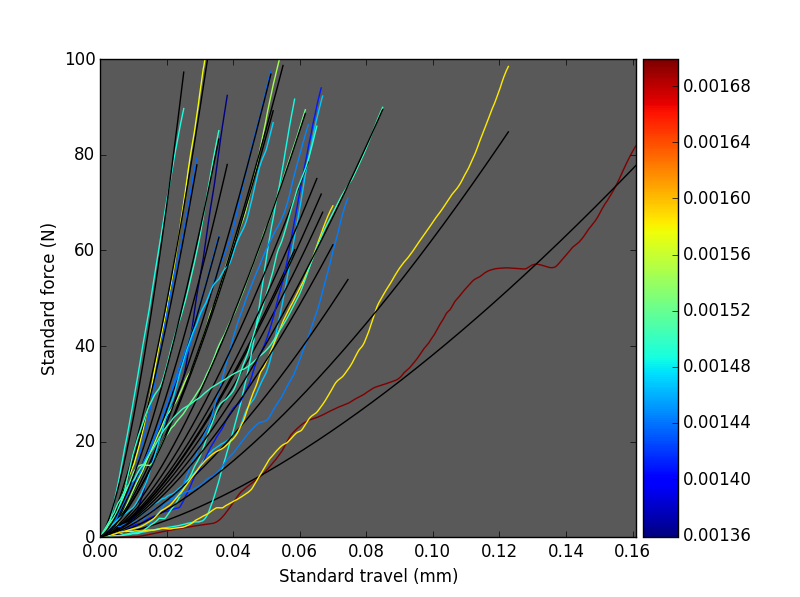
\includegraphics[width=\textwidth]{figures/nfri-1.5mm-hertz-colormap.png}
                \caption{$\bar{d}_p = 1.5$ mm}
                \label{fig:nfri-1.5-exp-hertz}
        \end{subfigure}
        \caption{Force-displacement curves for \lit~pebbles (in color) along with their Hertzian fits (in black) calculated with each pebble having a unique elastic modulus.}\label{fig:nfri-exp-hertz}
\end{figure}

The majority of the curves for two batches of \lit~pebbles analyzed (\Cref{fig:nfri-exp-hertz}) fit well to Hertzian curves with apparent elastic moduli. Apparent elastic moduli of the \lit~pebbles are given in \Cref{fig:nfri-E-plot}. Histograms of $\kappa$ for two batches of \lit~are given in \Cref{fig:nfri-kappa-hist}. The distributions for both batches of \lit~pebbles more closely resemble Snedecor's F distribution with many pebbles behaving with a very small $\kappa$, then a long tail of few pebbles with large $\kappa$.

\begin{figure}
        \centering
        \begin{subfigure}[b]{\doubleimagewidth}
                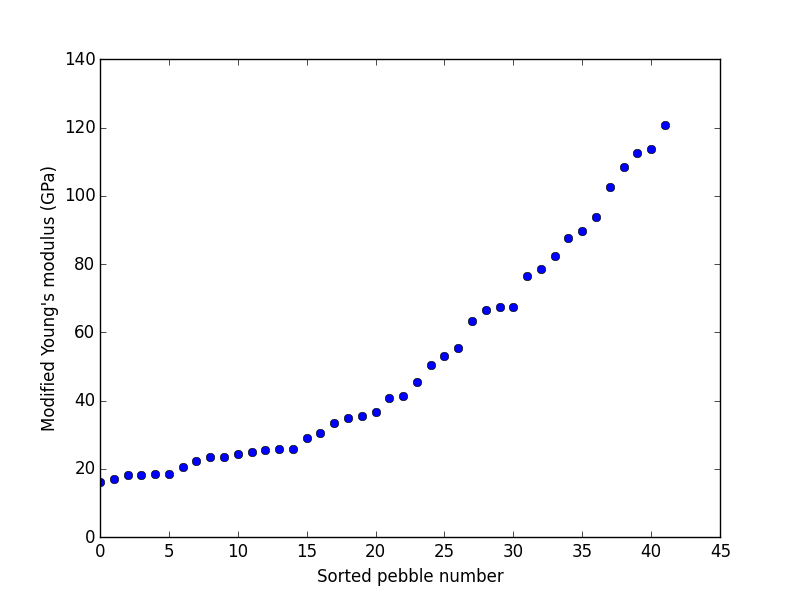
\includegraphics[width=\textwidth]{figures/nfri-1mm-E-plot.png}
                \caption{$\bar{d}_p = 1$ mm}
                \label{fig:nfri-1mm-E-plot}
        \end{subfigure}
        ~
        \begin{subfigure}[b]{\doubleimagewidth}
                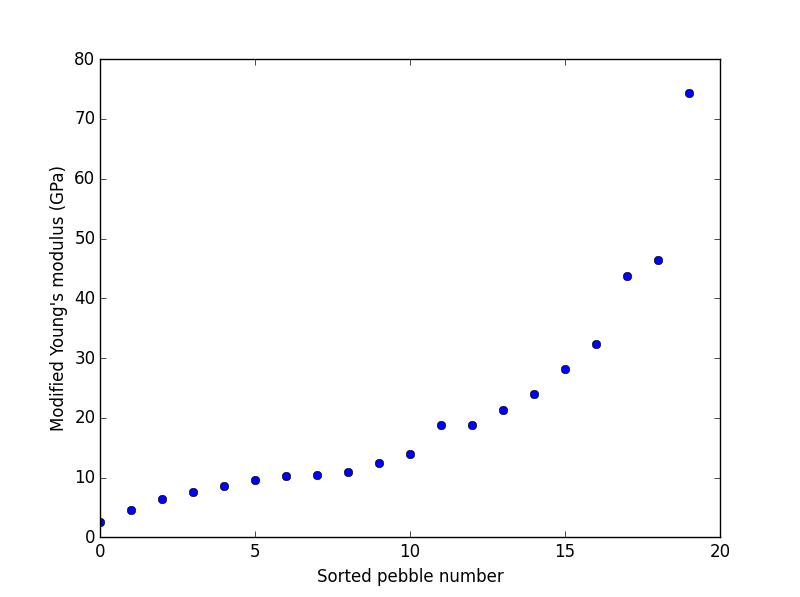
\includegraphics[width=\textwidth]{figures/nfri-1.5mm-E-plot.png}
                \caption{$\bar{d}_p = 1.5$ mm}
                \label{fig:nfri-1.5mm-E-plot}
        \end{subfigure}
        \caption{Distribution of modified elastic modulus for a batch of \lit~pebbles. All pebbles responded to compression with a elastic modulus well below the sintered pellet value of \si{126 GPa}.}\label{fig:nfri-E-plot}
\end{figure}

In \Cref{fig:nfri-kappa-dp-scatter} we see scatter plots of the pebble diameters against $\kappa$ values for the different batches of lithium ceramic pebbles. A Pearson Correlation value was calculated for each of the batches to quantify a correlation between diameter and $\kappa$. For the \lis~pebbles, we find $R = 0.198$ which is a weak positive correlation. For the \lit~pebbles we have $R = -0.385$ for $\bar{d}_p = 1$~mm and $R = -0.201$ for $\bar{d}_p = 1.5$~mm. Both of these are weakly negatively correlated. 

We hypothesize that manufacturing processes of pebbles leads to slightly different internal structures in the ceramic. Those differences yield stronger or weaker pebbles in a probability around a mean value, as seen in \Cref{fig:nfri-1-exp-fmax}. Different internal structure would then also cause each pebble to behave with different stiffness. Thus if the elastic modulus in \Cref{eq:contact-force} for the batch of pebbles had a probability distribution, rather than a single value, we can account for the variations in responses of \Cref{fig:nfri-exp-curves}. 


The results of these single pebble experiments indicate that the elastic modulus traditionally used in DEM simulations for ceramic pebble beds in solid breeders is incorrect. Numerical re-creations of the probability distribution curves will be used to apply $\kappa$ to pebbles in the ensemble. From the weak correlations between diameter and $\kappa$, we are free to ignore any diameter dependence when assigning $\kappa$ values in the DEM framework, especially in light of the current implementation of monodisperse pebble beds. Therefore, numerically, when assigning elastic moduli to the particles in the ensemble, the $\kappa$ distribution will be applied in a random fashion.

% \begin{figure}[ht]
% \centering
%     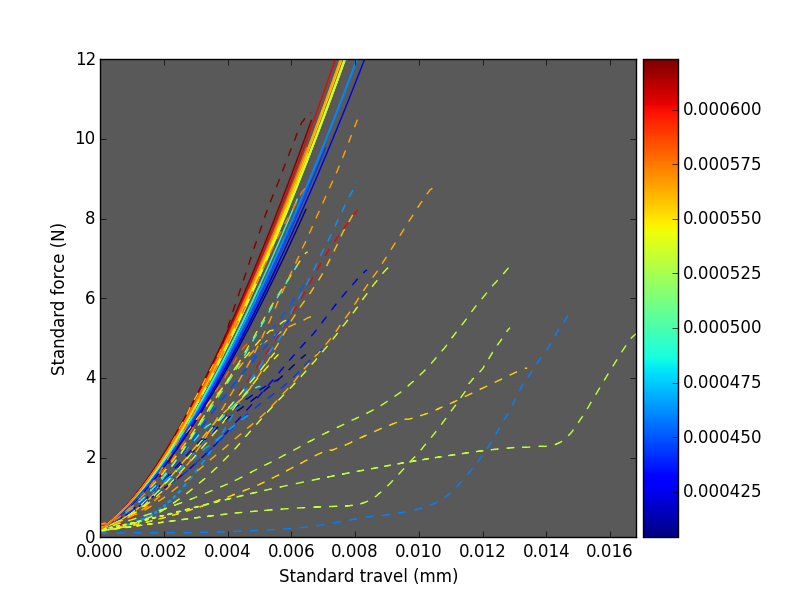
\includegraphics[width=\doubleimagewidth]{figures/fzk-data-w-ideal-hertz.png}
%     \caption{Dashed lines are \lis~pebbles of approximately \si{0.5 mm} diameter. Solid lines are the Hertzian (Eq.\ref{eq:contact-force}) responses based on each pebble's measured diameter.}
%     \label{fig:fzk-exp-colormap}
% \end{figure}


% \begin{figure}[ht]
% \centering
%     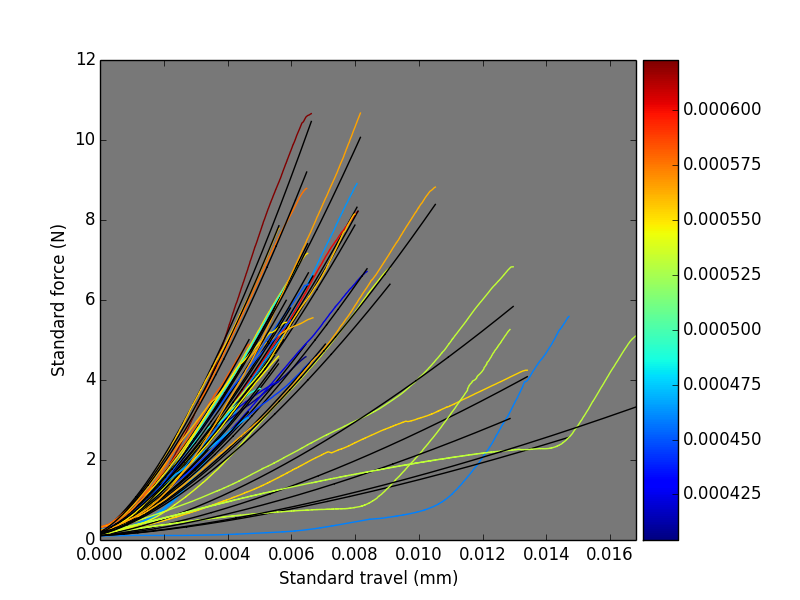
\includegraphics[width=\doubleimagewidth]{figures/fzk-hertz-colormap.png}
%     \caption{Force-displacement curves for \lis~pebbles (in color) along with their Hertzian fits (in black) calculated with each pebble having a unique elastic modulus.}
%     \label{fig:fzk-exp-hertz}
% \end{figure}


% \begin{figure}[ht]
% \centering
%     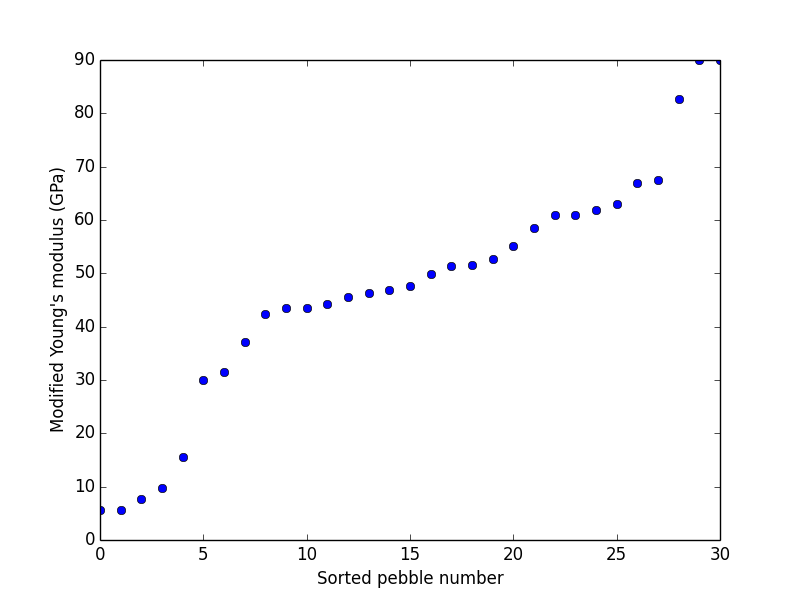
\includegraphics[width=\doubleimagewidth]{figures/fzk-E-plot.png}
%     \caption{Distribution of modified elastic modulus for a batch of \lis~pebbles. Most pebbles responded to compression with a elastic modulus well below the sintered pellet value of \si{90 GPa}.}
%     \label{fig:fzk-E-plot}
% \end{figure}


% \begin{figure}[ht]
% \centering
%     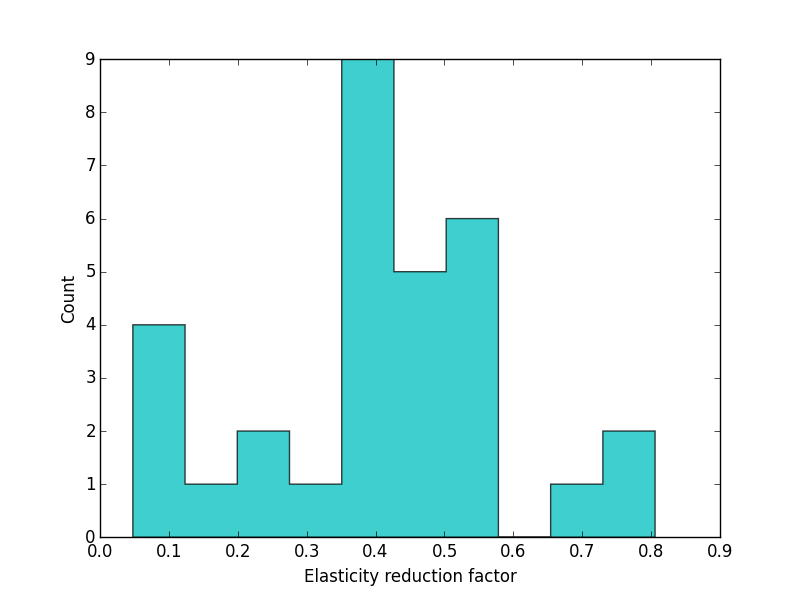
\includegraphics[width=\doubleimagewidth]{figures/fzk-kappa-histogram.png}
%     \caption{Histogram of $\kappa$ for a batch of \lis~pebbles. Most pebbles responded to compression with a elastic modulus well below the sintered pellet value of \si{90 GPa}.}
%     \label{fig:fzk-kappa-hist}
% \end{figure}

\begin{figure}
        \centering
        \begin{subfigure}[b]{\doubleimagewidth}
                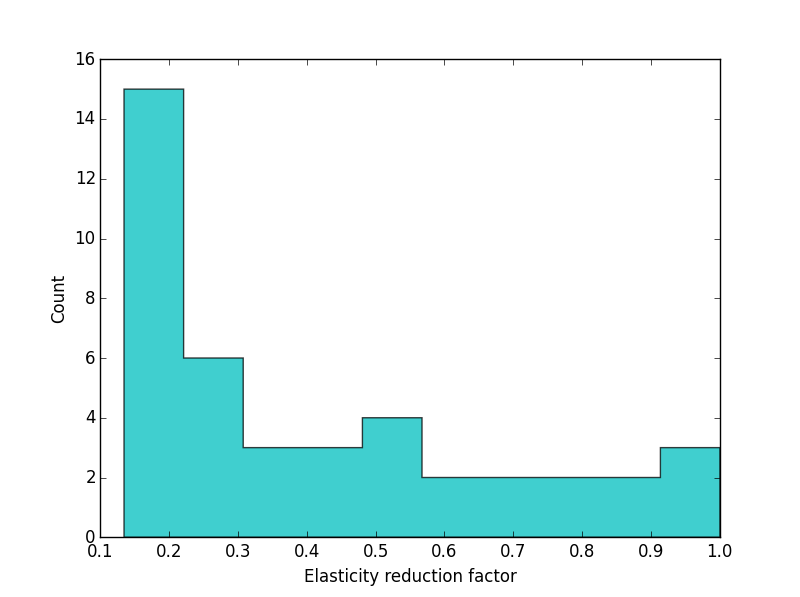
\includegraphics[width=\textwidth]{figures/nfri-1mm-kappa-histogram.png}
                \caption{$\bar{d}_p = 1$ mm}
                \label{fig:nfri-1mm-kappa-hist}
        \end{subfigure}
        ~
        \begin{subfigure}[b]{\doubleimagewidth}
                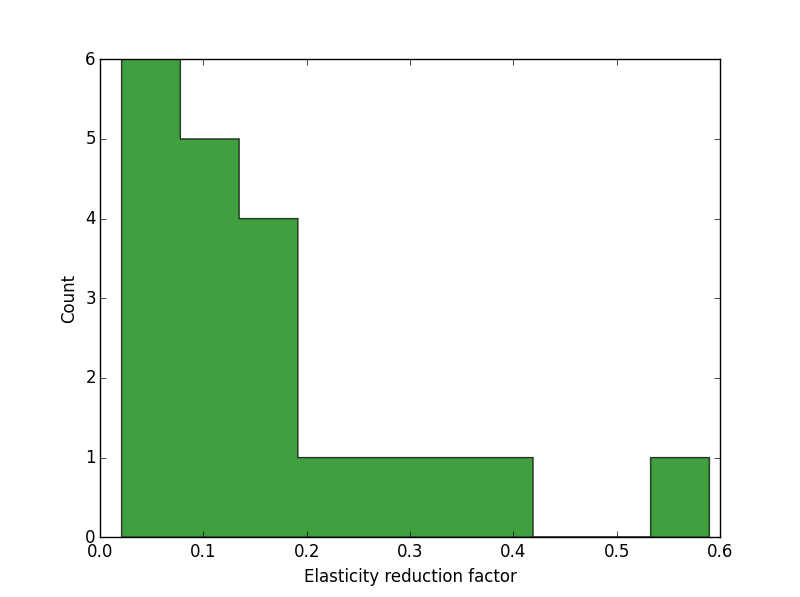
\includegraphics[width=\textwidth]{figures/nfri-1.5mm-kappa-histogram.png}
                \caption{$\bar{d}_p = 1.5$ mm}
                \label{fig:nfri-1.5mm-kappa-hist}
        \end{subfigure}
        \caption{Histogram of $\kappa$ for two batches of \lit~pebbles. All pebbles responded to compression with a elastic modulus well below the sintered pellet value of \si{126 GPa}.}\label{fig:nfri-kappa-hist}
\end{figure}


% \begin{figure}[!ht]
% \centering
%     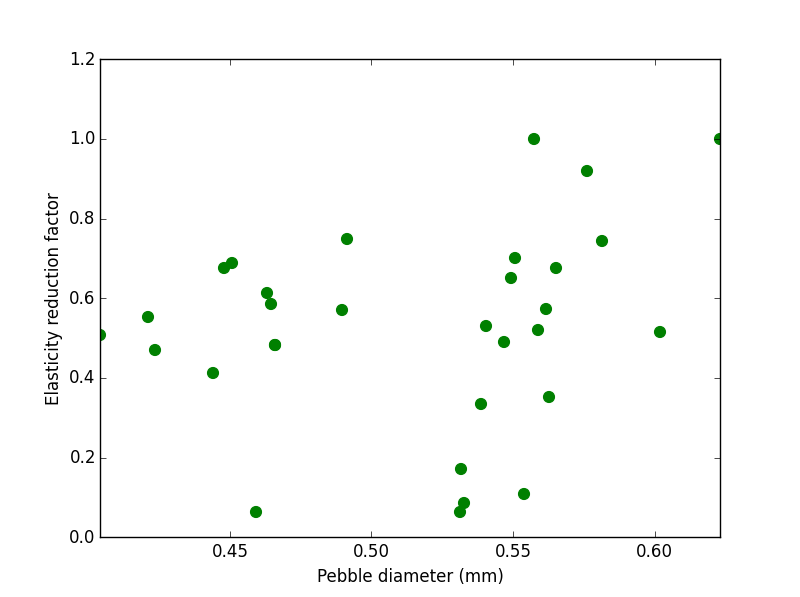
\includegraphics[width=\doubleimagewidth]{figures/fzk-kappa-dp-scatter.png}
%     \caption{Scatter of $\kappa$ against pebble diameter for a batch of \lis~pebbles showing almost no relationship between apparent stiffness and diameter.}
%     \label{fig:fzk-kappa-dp-scatter}
% \end{figure}

\begin{figure}
        \centering
        \begin{subfigure}[b]{\doubleimagewidth}
                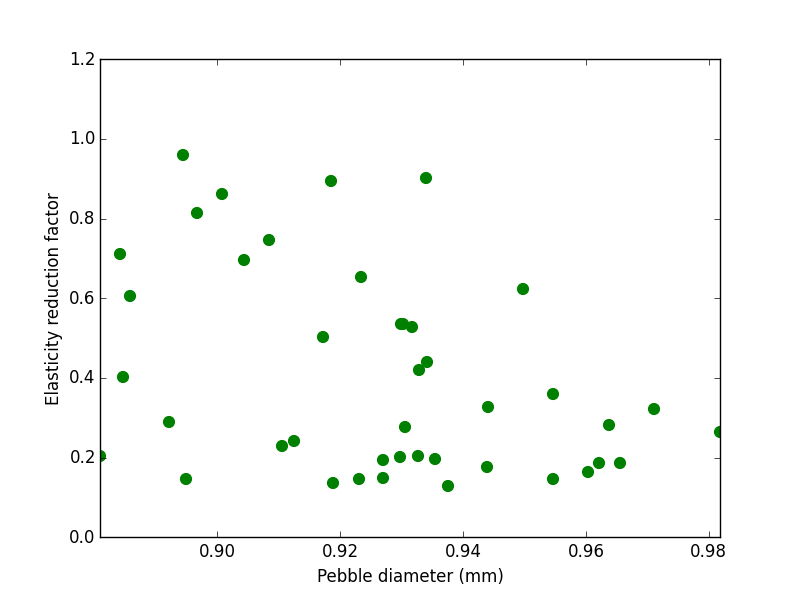
\includegraphics[width=\textwidth]{figures/nfri-1mm-kappa-dp-scatter.png}
                \caption{$\bar{d}_p = 1$ mm}
                \label{fig:nfri-1mm-kappa-dp-scatter}
        \end{subfigure}
        ~
        \begin{subfigure}[b]{\doubleimagewidth}
                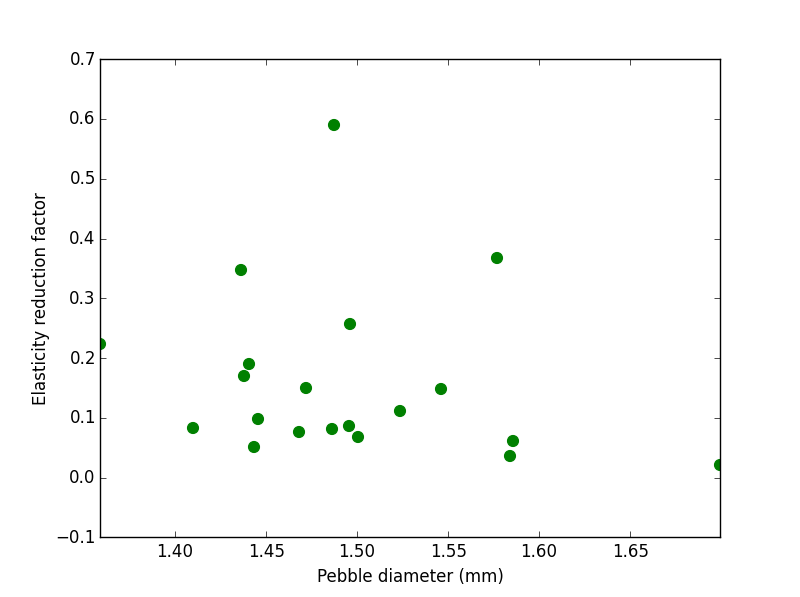
\includegraphics[width=\textwidth]{figures/nfri-1.5mm-kappa-dp-scatter.png}
                \caption{$\bar{d}_p = 1.5$ mm}
                \label{fig:nfri-1.5mm-kappa-dp-scatter}
        \end{subfigure}
        \caption{Scatter of $\kappa$ against pebble diameter for two batches of \lit~pebbles showing almost no relationship between apparent stiffness and diameter.}\label{fig:nfri-kappa-dp-scatter}
\end{figure}

\FloatBarrier


%~~~~~~~~~~~~~~~~~~~~~~~~~~~~~~~~~~~~~~~~~~~~~~~~~~~~~~~~~~~~~~~~~~~~~~~~~~~~~~~~~~~~~~~~~~~~~~~~~~~~~~~~~~~
% new subsection
%~~~~~~~~~~~~~~~~~~~~~~~~~~~~~~~~~~~~~~~~~~~~~~~~~~~~~~~~~~~~~~~~~~~~~~~~~~~~~~~~~~~~~~~~~~~~~~~~~~~~~~~~~~~
\subsection{Elastic Modulus Influence on Mechanical Response of Pebble Beds}\label{sec:dem-studies-youngs-modulus}

Proper calculation of normal force in DEM simulations is critical for accuracy in heat transfer modeling, as seen in \Cref{eq:cheng-modification-batchelor}, as well as accuracy in predictions of pebble crushing, as will be shown in \Cref{sec:failure-study}. We showed in the previous section that Hertzian contact is generally valid for describing pebble interactions. The Hertzian force is linearly proportional to the pair elastic modulus of contacting spheres. Based on the softening coefficient, $\kappa$, values found in \Cref{sec:exp-reduction-factor}, the apparent elastic moduli of \lis~and \lit~are, on average, less than half the values given for sintered materials in literature. For the case of \lit, the average value was closer to only 10\% of the value from literature. Thus the actual contact forces in pebble beds may be 10\% of the values found from DEM simulations with incorrect elastic modulus! In this section, we compare a number of pebble beds modeled with DEM using different elastic moduli. 

We first simulate uniaxial compression tests on pebble beds. One set of beds will be composed of pebbles with the single elastic modulus from literature and the other set will be composed of pebbles with a distribution of elastic moduli that fit the distribution from experiments. The second set of numerical experiments will simply compare the effective thermal conductivity of pebble beds as a function of elastic modulus.
%~~~~~~~~~~~~~~~~~~~~~~~~~~~~~~~~~~~~~~~~~~~~~~~~~~~~~~~~~~~~~~~


\subsubsection{Uniaxial Compression Simulations: Numerical Setup}
%In pebble bed breeder units, the stresses on the pebble regions are a result of thermal expansion of the relatively hot pebbles contained by relatively cool container walls. This process is a function of the coefficient of thermal expansion of the pebbles and their elevated temperature; the confined strain relates to a stress. 
The pebble beds are modeled as undergoing a standard uniaxial compression up to 6 MPa while measuring the macroscopic stress-strain for some parametrically varied pebble beds. At the moment of maximum stress, we can investigate the differences in contact forces of the different pebble beds.

Our pebble ensemble is composed of \SI{0.5}{\milli\meter} diameter \lis~pebbles. The pebble beds are initiated and packed in the same manner as \Cref{sec:dem-benchmark}. There are two main bed groups. Set A: three beds (A.1-3) containing a single type of pebble with $E$ = \si{90 GPa}. Set B: four beds (B.1-4) containing ten types of pebbles with their elastic modulus assigned in a discrete, random way to satisfy the distribution seen from experimental data. For the DEM study, \lis~pebbles are fit with a Weibull distribution of shape parameter $\sigma = 1.6$ where the average stiffness was $\bar{E} = 49$~GPa. The description of the two sets of pebble beds is visually represented in \Cref{fig:dem-types}. The pebble bed geometry was also the same used in the study of Ref.~\cite{VanLew2014}~: two virtual walls in the x-direction located at $x_\text{lim} = \pm 20 R_p$, periodic boundaries at the limits of $y_\text{lim} = \pm 15 R_p$, and a total of 8000 pebbles packed into the volume to an approximate height of $z_\text{lim} = 20 R_p$.

Among both sets, a parametric study was done on pebble radius and coefficient of friction. The radii of pebbles in beds A.1, A.2, B.1, and B.2 were constant at $R_p$=.25 mm. The radii of pebbles in beds A.3, B.3, and B.4 followed a Gaussian distribution about $\bar{R}_p$ = 0.25 mm: $\mu_d = R_p$ and $\sigma_d = R_p$. The coefficient of friction was set at $\mu = 0.2$ for beds A.1, A.3, B.1, and B.3; the coefficient of friction was $\mu = 0.3$ for beds A.2, B.2, and B.4.


\begin{figure}[t]
  \centering
  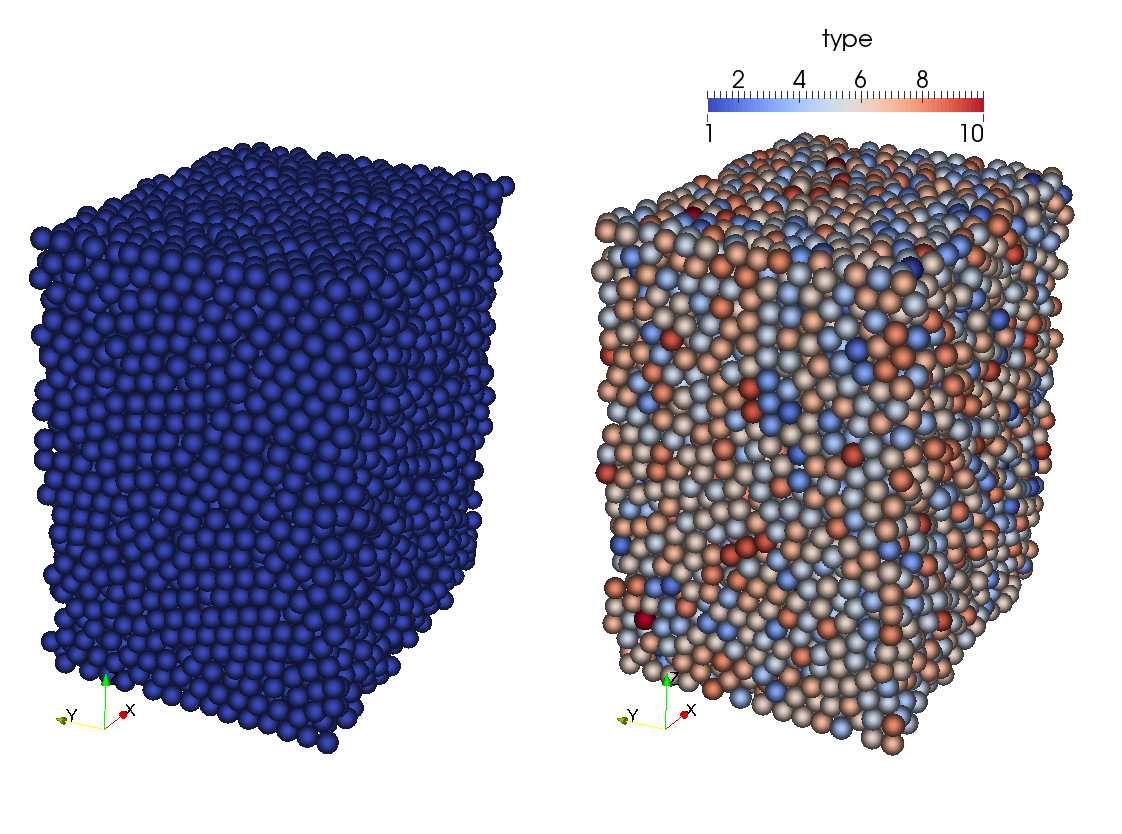
\includegraphics[width=\singleimagewidth]{figures/DEM-types}
  \caption{On the left, set A, a pebble bed with a single type, of $E = 120$ GPa. On the right, set B, is a pebble bed with 10, randomly distributed types; each type corresponds to a reduced, apparent elastic modulus as derived from experimental data.}\label{fig:dem-types}
\end{figure}



%~~~~~~~~~~~~~~~~~~~~~~~~~~~~~~~~~~~~~~~~~~~~~~~~~~~~~~~~~~~~~~~
\subsubsection{Uniaxial Compression Simulations: Results}


A constant-velocity, uniaxial compression was applied to the pebble beds. A single cycle up to \SI{6}{\mega\pascal} then down to \SI{0}{\mega\pascal} was used on all the beds. The macroscopic measurements of stress-strain are shown for all the pebble beds in \Cref{fig:stress-strain}.

\begin{figure}[t]
  \centering
  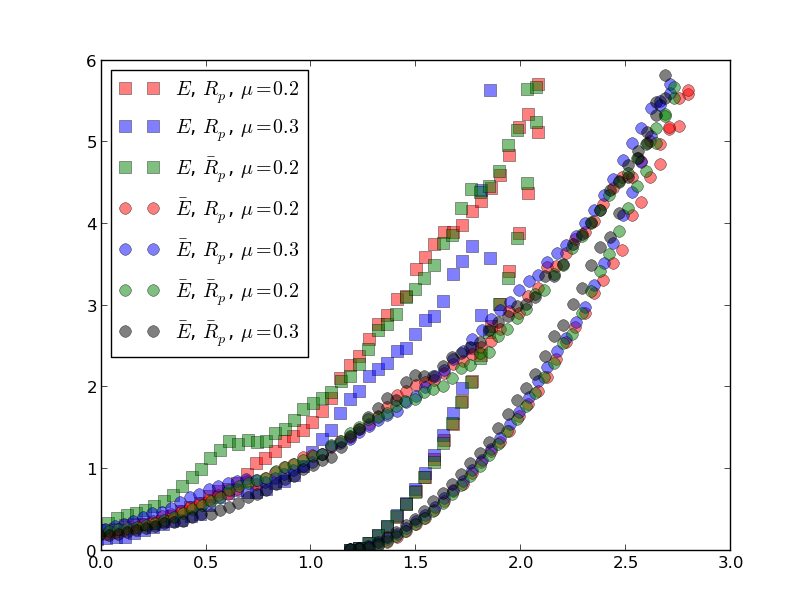
\includegraphics[width=\singleimagewidth]{figures/stress-strain}
  \caption{Stress-strain responses of pebble beds with: squares, constant elastic modulus; and circles, Gaussian distribution of elastic modulus. The constant elastic modulus beds all had much firmer responses for all parametric cases studied here.}\label{fig:stress-strain}
\end{figure}

Naturally, the pebble beds with smaller elastic�s modulus (with circle markers) are more compliant to external loads. The result is true regardless of the coefficient of friction or distribution of pebble radius studied here. Group B moved to an average strain of about 2.6\% at \SI{6}{\mega\pascal}, by comparison the beds of Group A only had strained 1.9\% on average to reach the same stress. Among the beds of each group, pebble beds with constant radius pebbles behaved virtually the same as similar pebble beds with a Gaussian distribution on radius. An increase in the coefficient of friction had a moderate impact on the overall stress-strain response. 


The parametric study here shows that the largest contributor to stress-strain response is the elastic�s modulus. The coefficient of friction and radius distribution had comparatively insignificant influence. A pebble bed geometry more directly comparable to oedometric compression experiments should be used to allow direct comparison and validation of the numerical models.


At the point of peak stress for each bed, DEM results are used to visualize the distribution of contact forces among all pebbles in the ensemble. A plot of the probability distributions of all the beds together, \Cref{fig:all-contact-forces}, shows that the majority of the contacts in all the beds are equally small. There are a few overall trends we observe from the results however. The pebble beds with the constant elastic modulus are always higher for their comparable version with distributed elastic modulus. For pebble beds with comparable elastic moduli and radii, higher coefficients of friction generally have higher peak contact forces. Pebble beds' radius distributions have much less impact on peak contact forces than either coefficient of friction or elastic�s modulus. Another method of comparing overall contact force distributions is to consider predictions on pebble cracking which assigns a strength value at random to pebbles in the bed (details are given in \Cref{sec:exp-reduction-factor}). At the point of maximum stress, this is done and the results are shown in \Cref{tab:num-crush-percent}.

While overall the predicted number of broken pebbles is small, we compare similar parameteric pebble beds and in each case pebble beds with modified elastic�s modulus overall predict smaller percentages of broken pebbles. Pebble crushing is a major topic for the overall evaluation of the feasibility of ceramic pebble beds in fusion reactors. This study reveals that past DEM work on pebble crushing, such as Ref.~\cite{Annabattula2012a,Annabattula2014,Zhao2013}, were likely over-predicting the extent of crushing if the elastic modulus used in the study was much larger than the realistic response of individual pebbles.

\begin{figure}[t]
  \centering
  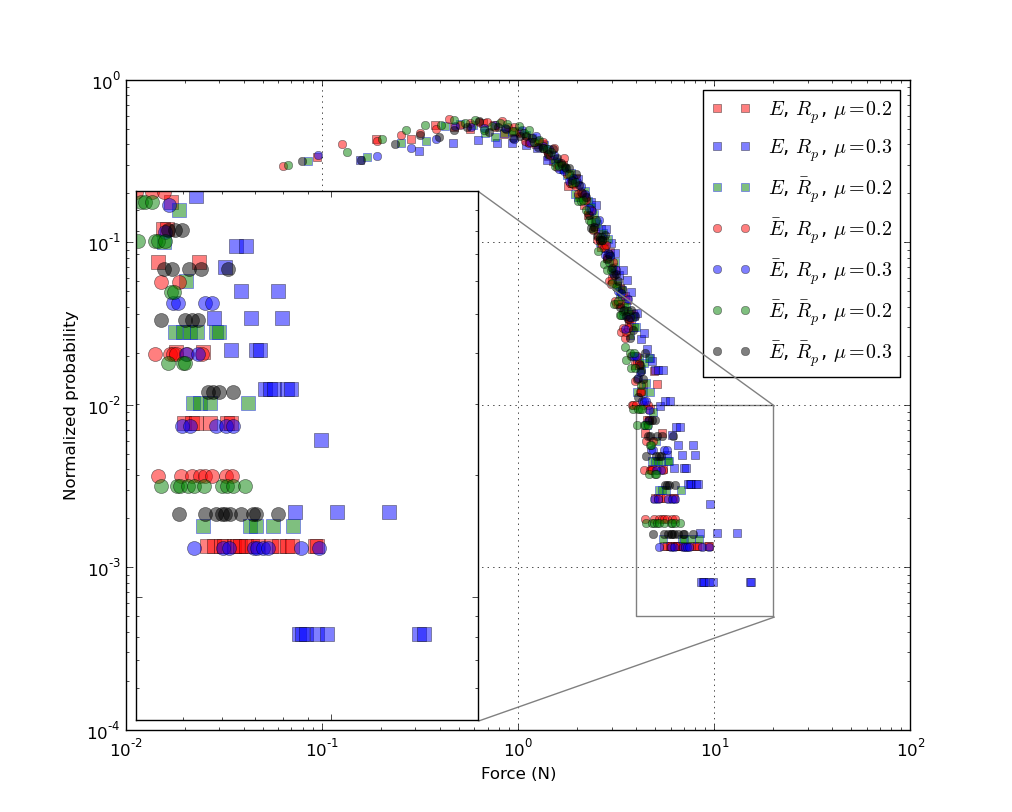
\includegraphics[width=\singleimagewidth]{figures/all-contact-forces}
  \caption{Probability distribution of contact forces in all the pebble beds studied here. Elastic moduli value is the largest contributor to higher peak contact forces among pebbles.}\label{fig:all-contact-forces}
\end{figure}


\begin{table}[t]
\caption{Comparisons for the two styles of elastic moduli used in the study. }
\label{tab:num-crush-percent}
\centering
\resizebox{0.45\textwidth}{!}{
\begin{tabular}{llS[table-format=3.2]}
\toprule
Bed label		& 		Parameters 								&	\text{Predicted crushed}			\\
				& 												&	\multicolumn{1}{r}{\text{\%}}		\\\otoprule
A.1				& 		$E$, $R_p$, $\mu = 0.2$          		&	0.3									\\\midrule
A.2				& 		$E$, $R_p$, $\mu = 0.3$     			&	1.0									\\\midrule
A.3				& 		$E$, $\bar{R}_p$, $\mu = 0.2$			&	0.9									\\\midrule
B.1				& 		$\bar{E}$, $R_p$, $\mu = 0.2$			&	0.6									\\\midrule
B.2				& 		$\bar{E}$, $R_p$, $\mu = 0.3$			&	0.8									\\\midrule
B.3				& 		$\bar{E}$, $\bar{R}_p$, $\mu = 0.2$		&	0.4									\\\midrule
B.4				& 		$\bar{E}$, $\bar{R}_p$, $\mu = 0.3$		&	0.7									\\\bottomrule
\end{tabular}}
\end{table}



% \subsubsection{elastic Modulus Influence on Heat Transfer: Numerical Setup}
% \subsubsection{elastic Modulus Influence on Heat Transfer: Results}



%~~~~~~~~~~~~~~~~~~~~~~~~~~~~~~~~~~~~~~~~~~~~~~~~~~~~~~~~~~~~~~~~~~~~~~~~~~~~~~~~~~~~~~~~~~~~~~~~~~~~~~~~~~~
% new subsection
%~~~~~~~~~~~~~~~~~~~~~~~~~~~~~~~~~~~~~~~~~~~~~~~~~~~~~~~~~~~~~~~~~~~~~~~~~~~~~~~~~~~~~~~~~~~~~~~~~~~~~~~~~~~
% \subsection{Conclusions of elastic Modulus Study}










\FloatBarrier

%%%%%%%%%%%%%%%%%%%%%%%%%%%%%%%%%%%%%%%%%%%%%%%%%%%%%%%%%%%%%%%%%%%%%%%%%%%%%%%%%%%%%%%%%%%%%%%%%%%%%%%%%%%%
%%%%%%%%%%%%%%%%%%%%%%%%%%%%%%%%%%%%%%%%%%%%%%%%%%%%%%%%%%%%%%%%%%%%%%%%%%%%%%%%%%%%%%%%%%%%%%%%%%%%%%%%%%%%
%
% new section
%
%%%%%%%%%%%%%%%%%%%%%%%%%%%%%%%%%%%%%%%%%%%%%%%%%%%%%%%%%%%%%%%%%%%%%%%%%%%%%%%%%%%%%%%%%%%%%%%%%%%%%%%%%%%%
%%%%%%%%%%%%%%%%%%%%%%%%%%%%%%%%%%%%%%%%%%%%%%%%%%%%%%%%%%%%%%%%%%%%%%%%%%%%%%%%%%%%%%%%%%%%%%%%%%%%%%%%%%%%
\section{Pebble Damage Modeling}\label{sec:failure-study}

To address pebble damage, there are two major modeling tasks: (i) predictive models for pebble crush events and (ii) modeling fragmentation after a crush event. For (i), the task is to develop a model to relate inter-particle pebble forces in an ensemble to measured crush loads of pebbles from experiments. Appendix \Cref{sec:pebble-crush-prediction} discusses predictive models developed in the fusion community as well as other theory behind a predictive model developed recently at UCLA. To address (ii), models must exist which simulate damage pebbles; \textit{i.e.} a scheme to treat a cracked, shattered, or crushed pebble in the assembly as small particles, removed particles, or particles with modified material properties.

Modeling of `crushed pebbles' in numerical assemblies has been attempted by a number of researchers. In most cases, indirect changes to the simulation are done with the hope of matching macroscopic features of beds that are observable in assemblies with damaged pebbles. In work by Marketos and Bolton, they treated a crushed pebble very similar to Van Lew\etal; when a pebble was damaged it was removed completely from the assembly.\cite{Marketos2007,VanLew2014} Marketos and Bolton study the stress-strain response of a pebble bed with a predictive crushing routine while Van Lew\etal~studied the effective thermal conductivity of a damaged pebble bed.

Annabattula\etal, noting the computationally expensive approach of modeling small fragments, introduced damaged pebbles \textit{via} reduction in elastic modulus.\cite{Annabattula2012a} Annabattula\etal~was also interested in the mechanics of the pebble bed with the presence of crushable materials. The study highlighted the differences in behavior of assemblies with different failure criteria and initial packings. From \Cref{fig:annabattula-stress-strain}, results are qualitatively similar to the stress-strain curves depicted by Marketos\etal.

\begin{figure}[ht]
\centering
	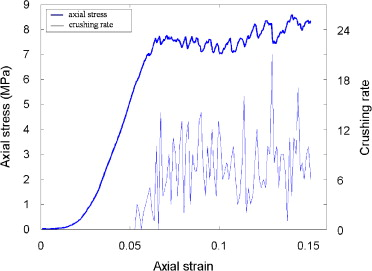
\includegraphics[width=\singleimagewidth]{figures/markets-bolton-stress-strain-crushing.jpg}
	\caption{Stress-strain response of a pebble bed with crushed pebbles modeled with removal of pebbles from assembly. Reproduced from Ref.~\cite{Marketos2007}}
	\label{fig:marketos-bolton-stress-strain}
\end{figure}

\begin{figure}[ht]
\centering
	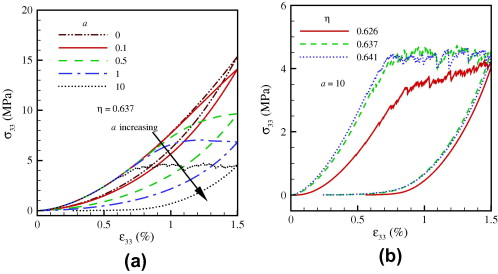
\includegraphics[width=\singleimagewidth]{figures/annabattula-stress-strain-crushing.jpg}
	\caption{Stress-strain response of a pebble bed with crushed pebbles modeled with reduction in elastic modulus with varying failure criteria. Reproduced from Ref.~\cite{Annabattula2012a}}
	\label{fig:annabattula-stress-strain}
\end{figure}


\begin{figure}[ht]
\centering
	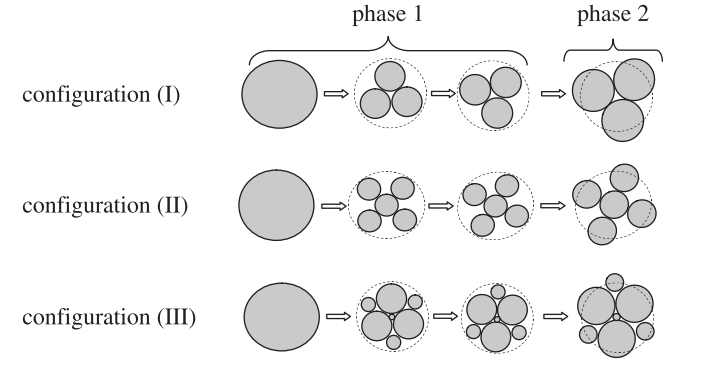
\includegraphics[width=\singleimagewidth]{figures/ben-nun-configurations}
	\caption{Configurations of fragmentation used in the study of Ref.~\cite{Ben-Nun2010a}}
	\label{fig:ben-nun-configurations}
\end{figure}


Ben-Nun\etal~studied the effects of fragmentation in two dimensional DEM studies of compressed packings.\cite{Ben-Nun2010,Ben-Nun2010a} In two dimensions, they were able to introduce small fragments after a crush event without excessive computational overhead. Under compression, they observed small fragments rearranging into smaller pores, giving rise to new force chains, until ultimately for a given initial volume an asymptotic limit is reached where fracture effectively stopped.\cite{Ben-Nun2010a} More important than his conclusions on self-organization in highly fragmented volumes were his observations that were similarly made here. In essence, any attempt to prescribe spherical fragments within the surface of a parent sphere will always fail to satisfy mass conservation (except in the limit of the fragment radius approaching 0). In order to resolve this situation Ben-Nun\etal~conserve the mass by inserting fragments in two phases: first, non-overlapping fragments are prescribed and randomly inserted, second, a rapid linear expansion is then introduced in the second phase to gain back the overall solid mass. Our approach, to be discussed soon, will be seen to be quite similar.

The importance of mass conservation in modeling ceramic pebbles beds for fusion is critically important to conserve energy in pre- and post-fragmentation systems. In the first study of Van Lew\etal~, where broken pebbles were removed from the system, energy input into two systems being studied were not dissimilar. This is quantified as follows. The total energy pouring into the non-damaged system is
\begin{equation}
	E_h = \frac{q'''_\text{nuc} V_\text{peb} N}{V_\text{bed}}
\end{equation}
where $N$ is the total number of pebbles of volume $V_\text{peb}$ that exist in the pebble bed of volume $V_\text{bed}$. After a crushing event, when pebbles are removed, the total amount of energy is
\begin{equation}
	E_h' = \frac{q'''_\text{nuc} V_\text{peb} \eta N}{V_\text{bed}}
\end{equation}
where $\eta$ is the percent of crushed pebbles. Obviously then, the ratio of the two heating rates is\begin{equation}
	\frac{E_h'}{E_h} = 1 - \eta
\end{equation}
and the energy deposited is not balanced between a virgin bed and one with crushed pebbles.

To continue the discussion of mass conservation of spherical packings, we consider how many fragments of a given radius would need to be inserted to conserve mass. In terms of DEM spheres we strictly wish to conserve mass between a solid pebble of radius $R_p$ and the crushed fragments of radius $R_c$. Thus the number of crushed fragments (spheres) per crushed pebble is
\begin{equation}\label{eq:nc-crushed-fragments}
	N_c = \left(\frac{R_c}{R_p}\right)^{-3}
\end{equation}

The number of fragments goes like the inverse of radius ratio to the third power; the number of crushed fragments to represent a single crushed pebble increases rapidly as the fragments shrink. The relationship between radius ratio and number of fragment particles is given in \Cref{fig:fragment-count}. Note that in the DEM simulation, it is impossible to insert fractions of a particle so the number of fragment pebbles is rounded to the nearest integer in the table. While the large numbers of fragments are computationally expensive to model, they are not prohibitive at least down to $R_c/R_p = 0.20$, as will be seen later.

\begin {table}[htp] %
\caption{Example values of the particle crush fragments, $N_c$, necessary to replace a single crushed particle and obey conservation of mass (fragment number is rounded to nearest integer).}
\label {tab:rstar-Nc} \centering %
\begin {tabular}{ S[table-format=3.2]S[table-format=3.2] }
\toprule
$R_c/R_p$ 						& $N_c$  				\\\otoprule
0.20                            & 125                   \\    
0.30                            & 37               \\
0.40                            & 16                   \\
0.50                            & 8                         \\
0.75                            & 2                \\\bottomrule
\end{tabular}
\end{table}


\begin{figure}[ht]
\centering
    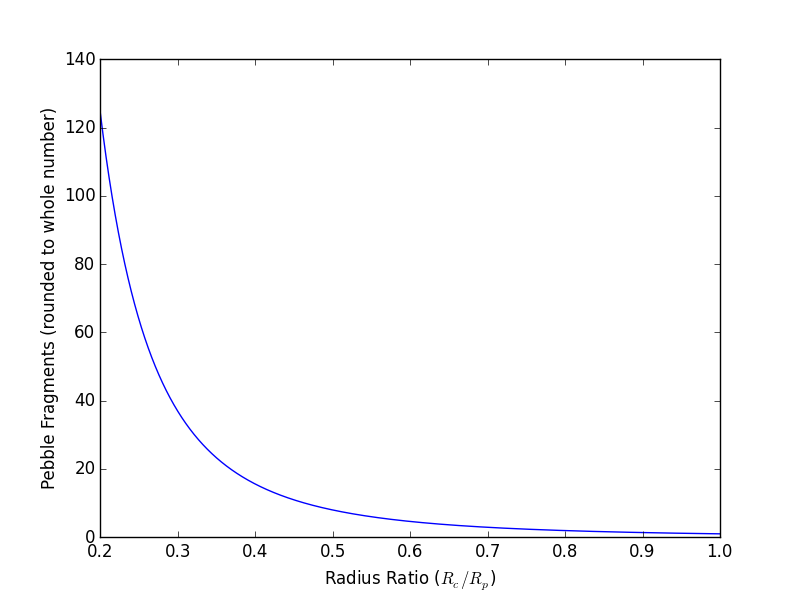
\includegraphics[width=\singleimagewidth]{figures/crush-fragments/pebble-fragment-count.png}
    \caption{Number of fragment pebbles necessary to conserve mass increases rapidly as the size of the radius ratio ($\frac{R_c}{R_p}$) decreases.}
    \label{fig:fragment-count}
\end{figure}

% In typical DEM simulations that can run within reasonable amounts of time on the machines available for this dissertation, a reasonable number of particles is on the order of \num{10000}. Significantly more and the run times become impractical for study. To show how quickly the number of particle fragments can quickly get out of hand in a simulation with small $R_c/R_p$, if we begin with \num{6000} pebbles and only 2\% break, with a radius ratio of $R_c/R_p = 0.2$, the number of pebbles to be added would be \num{15000}. The new particle fragments (less the crushed particles) plus the original would require \num{21000} particles in the system. In our simulations, we often test the effects on effective thermal conductivity at particle crush amounts of to 10\%. For the pebble bed mentioned here, that would mean \num{81000} particles in the system and it would be computationally taxing. The result is that, for the sake of computational times, the larger crush fragment radii are desired, \textit{i.e.} $R_c/R_p > 0.3$.
Aside from satisfying conservation of mass, we must physically insert the particle fragments into void space in the simulation domain. During the course of the simulation, when we choose to replace the pebble with the fragments, the only available room is the spherical void left over by the damaged pebble. As mentioned previously, without allowing overlap, the condition of mass conservation will never be satisfied. Then we may consider what precisely is the smallest size sphere that could hold non-overlapped spheres of given fragment radii.

Luckily, dense packing of spheres inside a larger sphere is an interesting mathematical problem and has been tackled by many mathematicians in the past. \href{http://www.randomwalk.de/sphere/insphr/spisbest.txt}{Hugh Pfoertner} keeps a compiled list of many solutions for a number of particles; many solutions are his are from Gensane.\cite{gensane2003dense} If we consider, for instance, that a radius ratio of $R_c/R_p = 0.3$ requires 37 particle fragments, then we can also find from Ref.~\cite{gensane2003dense} that 37 particles would have to be of radius 0.2406866 to fit into a single sphere of radius of unity. We defined the particle fragment radius as $R_c$, the original particle as $R_p$, and then the radius of sphere necessary to hold the $N_c$ fragments will be $R_N$, we can find a relationship between the volume of sphere $V_p$ and necessary volume $V_N$,
\begin{equation}
	r_1^* = \frac{R_c}{R_p}
\end{equation}
and
\begin{equation}
	r_2^* = \frac{R_c}{R_N}
\end{equation}
then 
\begin{equation}
	R_N = R_p \frac{r_1^*}{r_2^*}
\end{equation}
thus
\begin{equation}
	\frac{V_N}{V_p} = \left(\frac{r_1^*}{r_2^*}\right)^3
\end{equation}

Choosing a linearly spaced distribution of $r_1^*$ between 0 and 1, allows finding $N_c$ particles necessary to conserve mass. Then from the $N_c$ particles we can find from the database of sphere packing solutions the size of sphere that would be necessary to fit the $N_c$ particles. The calculations are carried out and shown in \Cref{fig:volume-ratio}. The data in Ref.~\cite{gensane2003dense} does not go above 72 spheres so we are limited to radius ratios above about $r_1^* > 0.24$.


\begin{figure}[ht]
\centering
    \includegraphics[width=\singleimagewidth]{figures/crush-fragments/fragment-volume-ratio.png}
    \caption{The volume necessary to house the particles of different radius ratios decreases toward unity as the radius ratio decreases. It is greater than 5 times the volume for large $r_1^*$.}
    \label{fig:volume-ratio}
\end{figure}

The plot of \Cref{fig:volume-ratio} shows that for particle fragments of reasonable numbers ($N_c\approx 20$ for $r_1^*\approx 0.3$), the volume necessary to fit the number of volume-conserving particles is greater than double the volume of the original sphere! Therefore from the point of view of having the physical space to insert the fragments, smaller sized fragments are ideal. To insert the few number of large particles would require disrupting the packing in the region of the damaged particle. From this discussion, we conclude that an upper size limit should approximately be $r_1^* = 0.3$. This result agrees with the work from Ben-Nun\etal~who only studied configurations with particles as large as $r_1^*=1/3$.\cite{Ben-Nun2010a}

Our approach for inserting mass-conserving fragments is in essence similar to that described by Ben-Nun\etal. Whereas they would insert fragments fully enveloped in the circle and then increase their radius up to a mass-conserving value, we insert mass-conserving spheres but allow extreme overlap in the first phase. In the second phase, we permit a relaxation of the overlap by enforcing a limit to the travel during integration with the velocity-Verlet scheme. After the fragments have slowly moved away from each other and reached a local equilibrium with their neighboring particles, we re-initiate standard velocity-Verlet integration of all the particles in the ensemble to allow fragmentation resettling.

In the next section, we see some sample pebble beds where fragmentation is induced to equal amounts but with varying fragmentation sizes. We will investigate such characteristics as disruption caused by large fragments and travel of small fragments during resettling.

\subsubsection{Example Beds with Fragmentation}

To study the effects on a pebble bed of different fragmentation schemes, we begin with a bed of \num{6875} particles and randomly crush 1\%. This was done with a range of fragments of size $r_1^* = [0.20, 0.25, 0.35, 0.50]$. The number of particles inserted for these different $r_1^*$ followed the from \Cref{eq:nc-crushed-fragments}. In the images of \Cref{fig:crush-settling-pictures-1},~\Cref{fig:crush-settling-pictures-2},~\Cref{fig:crush-settling-pictures-3}, and~\Cref{fig:crush-settling-pictures-4}, we see the initial packing of new particle fragments (in blue) settle into the interstitial gaps of the packing structure of original pebbles (yellow).


\begin{figure}[!ht]
	\centering
	\begin{subfigure}[b]{\doubleimagewidth}
		\centering
		\includegraphics[width=\textwidth]{figures/crush-fragments/0.20-1.png}
		\caption{initial}
	\end{subfigure}
	\begin{subfigure}[b]{\doubleimagewidth}
		\centering
		\includegraphics[width=\textwidth]{figures/crush-fragments/0.20-2.png}
		\caption{final}
	\end{subfigure}
	\caption{$N_c = 8594$, $N_\text{tot} = 15430$, $r_1^* = 0.20$. Side view of the packing arrangement and settling for different crush fragment sizes. The small crush fragments migrate far through the height of the bed. The yellow particles are the original pebbles and the blue are fragments inserted into the system after pebble crushing.}
\label{fig:crush-settling-pictures-1}
\end{figure}
\begin{figure}[!ht]
	\begin{subfigure}[b]{\doubleimagewidth}
		\centering
		\includegraphics[width=\textwidth]{figures/crush-fragments/0.25-1.png}
		\caption{initial}
	\end{subfigure}
	\begin{subfigure}[b]{\doubleimagewidth}
		\centering
		\includegraphics[width=\textwidth]{figures/crush-fragments/0.25-2.png}
		\caption{final}
	\end{subfigure}
	\caption{$N_c = 4400$, $N_\text{tot} = 11222$, $r_1^* = 0.25$. Side view of the packing arrangement and settling for different crush fragment sizes. The small crush fragments migrate far through the height of the bed. The yellow particles are the original pebbles and the blue are fragments inserted into the system after pebble crushing.}
\label{fig:crush-settling-pictures-2}
\end{figure}

\begin{figure}[!ht]
	\centering
	\begin{subfigure}[b]{\doubleimagewidth}
		\centering
		\includegraphics[width=\textwidth]{figures/crush-fragments/0.35-1.png}
		\caption{initial}
	\end{subfigure}
	\begin{subfigure}[b]{\doubleimagewidth}
		\centering
		\includegraphics[width=\textwidth]{figures/crush-fragments/0.35-2.png}
		\caption{final}
	\end{subfigure}
	\caption{$N_c = 1603$, $N_\text{tot} = 8393$, $r_1^* = 0.35$. Side view of the packing arrangement and settling for different crush fragment sizes. The bigger fragments remain largely in place. The yellow particles are the original pebbles and the blue are fragments inserted into the system after pebble crushing.}
\label{fig:crush-settling-pictures-3}
\end{figure}
\begin{figure}[!ht]
	\begin{subfigure}[b]{\doubleimagewidth}
		\centering
		\includegraphics[width=\textwidth]{figures/crush-fragments/0.50-1.png}
		\caption{initial}
	\end{subfigure}
	\begin{subfigure}[b]{\doubleimagewidth}
		\centering
		\includegraphics[width=\textwidth]{figures/crush-fragments/0.50-2.png}
		\caption{final}
	\end{subfigure}
	\caption{$N_c = 550$, $N_\text{tot} = 7358$, $r_1^* = 0.50$. Side view of the packing arrangement and settling for different crush fragment sizes. The bigger fragments remain largely in place. The yellow particles are the original pebbles and the blue are fragments inserted into the system after pebble crushing.}
\label{fig:crush-settling-pictures-4}
\end{figure}
\FloatBarrier


\begin{figure}[ht]
\centering
    \includegraphics[width=\singleimagewidth]{figures/crush-fragments/displacement-scatter-radius-ratios.png}
    \caption{After the particle fragments are inserted into the system they re-settle due to gravity and inter-particle forces. The small fragments travel much further throughout the bed than the large fragments.}
    \label{fig:displacement-scatter}
\end{figure}

The settling of crushing fragments is also visualized in \Cref{fig:displacement-scatter}. For this figure, the magnitude of displacement for all the crushed fragments is recorded based on the change between initial insertion location and final resting place. The displacement of the fragments is normalized against a pebble diameter and then a probability distribution is generated. Immediately obvious from \Cref{fig:displacement-scatter} is that larger fragments, $r_1^*=[0.35, 0.50]$ rarely travel beyond their original insertion point; very few particles have a normalized fragment settling distance larger than 1.0. In contrast, a good number of smaller fragments travel well beyond a single pebble diameter. In fact, 12\% of the fragments of size $r_1^* = 0.20$ travel more than 2 diameters before coming to rest. We will return to the effects of pebble fragment travel when we consider ITER-relevant configurations and pebble bed heating.

\begin{figure}[ht]
\centering
    \includegraphics[width=\singleimagewidth]{figures/crush-fragments/packing-fraction-height.png}
    \caption{For only 1\% of crushed pebbles, the re-settling of small pebble fragments has a small effect on the overall packing fraction of the pebble bed. In the inset, the main influence is seen in the slight increase of packing fraction within the first pebble radius of the floor.}
    \label{fig:fragment-packing-fraction}
\end{figure}

From \Cref{fig:displacement-scatter}, the impression then arises that the large displacement magnitudes of the small crush fragments may result in an overall less-dense bed with large increase in packing fraction near the floor where pebbles settle. For 1\% crushed pebbles, there is some observable changes to the local packing fraction near the floor of the pebble bed, but no appreciable changes elsewhere in the bulk. In \Cref{fig:fragment-packing-fraction}, the packing fractions of the four different pebble beds are given. We look closely at the distribution within the first pebble diameter (see inset of \Cref{fig:fragment-packing-fraction}) and see the small crush fragments have a small change to the local packing fraction as they settled onto the floor of the container.

\begin{figure}[!ht]
	\centering
	\begin{subfigure}[b]{\doubleimagewidth}
		\centering
		\includegraphics[width=\textwidth]{figures/crush-fragments/force-scatter-20.png}
		\caption{$r_1^* = 0.20$}\label{fig:fragment-contact-forces-20}
	\end{subfigure}
	\begin{subfigure}[b]{\doubleimagewidth}
		\centering
		\includegraphics[width=\textwidth]{figures/crush-fragments/force-scatter-25.png}
		\caption{$r_1^* = 0.25$}\label{fig:fragment-contact-forces-25}
	\end{subfigure}

	\begin{subfigure}[b]{\doubleimagewidth}
		\centering
		\includegraphics[width=\textwidth]{figures/crush-fragments/force-scatter-35.png}
		\caption{$r_1^* = 0.35$}
	\end{subfigure}
	\begin{subfigure}[b]{\doubleimagewidth}
		\centering
		\includegraphics[width=\textwidth]{figures/crush-fragments/force-scatter-50.png}
		\caption{$r_1^* = 0.50$}
	\end{subfigure}
	\caption{Contact force distributions throughout the pebble beds with different crush fragment sizes. Average forces in the bed are largely unaffected by the size of crushed particle fragments.}
\label{fig:fragment-contact-forces}
\end{figure}

\FloatBarrier

The last point to discuss is how the different size particles change the distribution of contact forces inside the ensemble. We plot the scatter of contact forces for all the pebbles in the ensemble in \Cref{fig:fragment-contact-forces}. We are most interested in the contact loads carried by the large particles that make up the force network after crush fragments are inserted into the ensemble. The small fragments, moving through the interstitial gaps, are not expected to carry much load. Therefore in the data processing for the subplot of \Cref{fig:fragment-contact-forces-20} and~\Cref{fig:fragment-contact-forces-25}, the vast number of small forces on the fragments are omitted in the average value of contact force. Opposingly, the larger fragments, $r_1^*>0.4$, are expected to be inserted firmly into the contact network and their contribution to the average value is included.

What we see in \Cref{fig:fragment-contact-forces} is that the average contact forces in the pebble bed remain mostly unchanged as a function of the size of the fragment radii. For all pebble beds, after the bed re-settles from the crushing event, the average contact forces (to the 1/3 power, which is the value important for heat transfer) are approximately $4.9\ N^{1/3}$. None of the beds have a maximum value greater than $9\ N^{1/3}$.



% %~~~~~~~~~~~~~~~~~~~~~~~~~~~~~~~~~~~~~~~~~~~~~~~~~~~~~~~~~~~~~~~~~~~~~~~~~~~~~~~~~~~~~~~~~~~~~~~~~~~~~~~~~~~
% % new subsection
% %~~~~~~~~~~~~~~~~~~~~~~~~~~~~~~~~~~~~~~~~~~~~~~~~~~~~~~~~~~~~~~~~~~~~~~~~~~~~~~~~~~~~~~~~~~~~~~~~~~~~~~~~~~~
% \subsection{Conclusions of Pebble Failure Modeling}






















%%%%%%%%%%%%%%%%%%%%%%%%%%%%%%%%%%%%%%%%%%%%%%%%%%%%%%%%%%%%%%%%%%%%%%%%%%%%%%%%%%%%%%%%%%%%%%%%%%%%%%%%%%%%
%%%%%%%%%%%%%%%%%%%%%%%%%%%%%%%%%%%%%%%%%%%%%%%%%%%%%%%%%%%%%%%%%%%%%%%%%%%%%%%%%%%%%%%%%%%%%%%%%%%%%%%%%%%%
%
% new section
%
%%%%%%%%%%%%%%%%%%%%%%%%%%%%%%%%%%%%%%%%%%%%%%%%%%%%%%%%%%%%%%%%%%%%%%%%%%%%%%%%%%%%%%%%%%%%%%%%%%%%%%%%%%%%
%%%%%%%%%%%%%%%%%%%%%%%%%%%%%%%%%%%%%%%%%%%%%%%%%%%%%%%%%%%%%%%%%%%%%%%%%%%%%%%%%%%%%%%%%%%%%%%%%%%%%%%%%%%%
\section{Summary of DEM Modeling of Solid Breeder Pebble Beds}
A transient, thermal discrete element method approach to studying heat transfer in pebble beds has been introduced. Use of the method is important for blanket researchers and designers because it allows one to interrogate solid-solid interactions in pebble beds and opens a window into the micro-mechanical world of pebble beds. The DEM method recreates the constriction of heat conduction through normal-force-dependent contact areas between pebbles and between pebble-walls in an ensemble. The approach also allows exploration of evolving packing structures that will occur during operation of a ceramic pebble bed in a solid breeder unit of a fusion reactor - in this case we specifically consider packing structure changes due pebble damage. DEM-based models provide us with the ability to understand, predict, and more importantly, ultimately avoid pebble damage and associated thermomechanical changes to pebble beds. 

Our DEM modeling of heat transfer was validated against experimental measurements of effective thermal conductivity of pebble beds in vacuum. The smooth-sphere approximation of pebbles was seen to over-predict the ability of pebbles to transport energy between contacts. Reductions in contact conductance due to roughness were shown to allow DEM models to approach experimental measurements. In the numeric models, we witnessed the phenomena of hot rattlers loosely settled in pebble beds and heating to a much higher degree then neighbors in the ensemble. If, in practice, the hot rattlers truly exist in solid breeders, it would be disadvantageous from the point of view of sintering or densification of pebbles leading to poorer tritium release. This observation strongly supported the need to include helium purge gas in models of thermal transport of pebble beds with DEM. 

A modified elastic modulus is shown to capture the observed scatter of elasticity of individual ceramic pebbles from experiments. The modified elastic Modulus is realized in DEM simulations with numeric re-creations of measured experimental elastic modulus distributions. The models applying modified elastic moduli predict more compliant pebble beds and smaller peak contact forces in beds and thus fewer crushed pebbles. Because normal contact forces between pebbles, a direct function of elastic modulus, are used to calculate pebble heat transfer and it is therefore imperative to have an accurate determination. The new approach to implementing elastic moduli in simulations is a necessary step towards more faithful DEM models.

In the case of a crushed pebble, a volume-conserving pebble fragmentation method is used to simulate a broken pebble. Smaller pebble fragments were seen to have the capability of traveling relatively long distances before re-settling. Redistribution of mass was seen in increased local packing fractions of beds. Nuclear heating of the beds will also be affected by mass redistribution and will be studied during applications of the models for ITER-relevant pebble beds.

We have demonstrated the usefulness of discrete element methods to model complex, transient, micro-mechanical interactions of pebbles in an ensemble and the concomitant heat transfer between them. Toward the goal of a complete model of thermal transport in solid breeder pebble beds, we must also take into account the slow-moving interstitial helium purge gas. In the next chapters, we will discuss augmentation of DEM models with two different schemes of helium flow models.





% from E section
% Variation in production techniques for ceramic pebbles have lead to batches of pebbles with slight differences in their ceramic microstructure, as evident in the wide distribution of crush loads reported in past studies, \textit{e.g.} Refs.~\cite{Zhao2012,Mandal2012a}. By the same token, the different microstructures should naturally lead to variation in elastic�s modulus. However up to now values of elastic�s modulus used in numerical models are taken from values measured for large sintered pellets of ceramic materials. Based on single pebble experiments and the application of Hertz theory, a technique for introducing a modified elastic�s modulus into DEM models has been proposed here. DEM simulations show the impact of modified pebble elasticity on both macroscopic measurements of stress-strain curves as well as mesoscopic measures of inter-pebble contact force -- with major implications for prediction of pebble crushing in ceramic pebble beds and macroscopic $\sigma-\epsilon$ responses. 

% Thus I conclude that in DEM numerical models for pebble damage, the modified elastic modulus with softening coefficients matching the probability density function from experiments must be used. In this way, we can expect a more realistic numerical tool to simulate pebble damage, bed rearrangement, and heat transfer.


% from damage section
% This section began with a review of past research efforts on predicting pebble crushing in an ensemble. There are two main theories for predicting pebble crushing: 1) the failure of a pebble is due to the summed total strain energy of all contacts acting on a pebble in an ensemble. 2) failure of a pebble is a localized event where the maximum contact force is the main agent for driving fragmentation. In our work, we have adopted the philosophy of the second approach. In short, I consider \textit{only the single largest contact force} on a pebble, irrespective of the number and magnitude of lesser contact forces on that pebble when predicting a crush event. With that in mind, we then showed how an equation can define critical contact forces for pebbles in a DEM simulation as defined by strain energy distributions measured from experimental campaigns on individual pebbles. The probabilistic nature of experimental measurements is naturally incorporated into the numeric computations \textit{via} recreations of the probability distribution functions matched to experimental measurements of strain energy.

% I also introduced a method for introducing crushed pebble fragments into an ensemble after pebble damage is predicted \textit{via} the above criteria. The method was necessary to enforce conservation of mass between pebble beds before and after the crushing event which is necessary for also balancing the energy deposition into the bed from volumetric heating before and after the crushing event. We then showed that fragments increase the computational time as $(1/r_1^*)^{1/3}$ while the necessary minimum volume for inserting the particles follows roughly as $(r_1^*)^{1/3}$. The size of fragments may still influence the overall transport of energy in the system but in terms of localizing heat deposition due to settling fragments in interstitial regions, I also showed that the local packing fraction was changed very little over the range of radius ratios tested. Thus from the point of view of capturing proper thermophysics of the system, there does not seem to be a strict sensitivity to choice of radius ratio of fragmentations. Choice of fragmentation size will be driven by consideration of other physical features, in this study we will continue to treat it as a free parameter during investigations of fragmentation impact.